\chapter{嵌入式系统的建模与验证}
\label{cha:modeling}

形式化模型是否适合应用于形式化建模与验证,除了取决于其自身的表达能力、验证能力外,还取决于它的易用性。不同于自动机、Petri 网等图形化模型,重写模型作为一种代数模型,其抽象的形式给建模人员的使用过程带来了额外的理解成本。本章通过提出一套针对嵌入式系统特性的建模方法,来提高规范化条件重写模型作为一种建模模型的易用性。基于语义映射,该建模方法可以在工具集 Maude 中予以实现。利用该建模方法,我们对两个真实的、经过大量测试的嵌入式系统进行了行为建模,并对其模型应用了模型检测等验证技术,成功地发现系统中存在未被测试检测到的缺陷。结果表明该方法在实际应用中具有可行性。

\section{引言}

随着嵌入式系统在生产、生活中越来越广泛的应用,嵌入式系统与我们的关系越来越紧密。特别是嵌入式系统在诸如交通运输、医疗系统、金融系统等安全攸关系统中扮演的重要角色,使其安全性、可靠性、正确性保障与我们的生命财产安全息息相关。

形式化建模与验证是提高嵌入式系统可靠性与安全性的重要方法之一。通过对嵌入式系统的行为进行建模,得到可以描述该系统行为的形式化模型。然后利用支持该模型的相关工具,对模型进行仿真、测试或形式化验证,从而检查该模型的行为是否满足开发人员的预期,进而反映原系统的行为是否满足用户的需求。

嵌入式系统的其中一个特点是具有高度并发性,这主要体现在三个方面。第一,由于嵌入式系统通常由硬件与软件协同完成其功能,硬件系统所具有的并发性不可忽视。其次,由于现代嵌入式系统处理单元逐渐变得强大,使得嵌入式软件日趋复杂。软件部分不仅仅限于完成单一任务,而且还可以搭载操作系统对复杂任务进行协调调度。软件部分的多线程进一步增加了嵌入式系统的并发性。第三,大型嵌入式系统一般由多层次构成,底层组件作为上层系统的一部分,与其它嵌入式组件协作共同完成复杂的功能,这造成了系统层面的并发性。

作为自带并发语义的一种形式化模型,重写模型及其扩展在近年来作为一种系统建模模型受到越来越多的关注,被应用到硬件描述、网络协议、安全协议等领域中~\cite{DBLP:journals/jlp/Meseguer12,DBLP:journals/iandc/MeseguerR13}。若要将其应用于嵌入式系统的实际建模验证项目,除了需要扩展现有模型提升其对软件顺序行为的描述能力外,仍需要面临两方面的挑战:
\begin{enumerate}
\item \textbf{建模方法:} 与基于状态的形式化模型(如自动机)不同,重写模型是基于抽象的项表达式与规则的。如何将重写模型的这些抽象元素与嵌入式系统的状态及复杂行为一一对应起来,需要一套系统的建模方法进行指导。
\item \textbf{工具支持:} 在根据建模方法对目标嵌入式系统进行建模,得到其对应的重写模型后,从应用的角度,我们需要一套工具支持该模型的分析与验证,否则建模毫无意义。
\end{enumerate}

本章基于第~\ref{cha:normalrewriting} 章提出的规范化条件重写模型,提出了一套系统建模方法,并针对嵌入式系统所具有的若干特性,如层次结构、高度并发、并发行为与顺序行为并存、系统结构动态变化、实时性等,将该建模方法进一步细化。基于已有的重写工具集 Maude,我们将本章提出的建模方法在 Maude 中予以实现,并通过两个真实的应用案例,验证了该方法的可行性与实用性。

本章其余部分组织结构如下:第~\ref{s:modeling-related} 小节简述基于重写模型的系统建模验证相关工作;第~\ref{s:modeling} 小节基于规范化条件重写模型,提出嵌入式系统的建模方法;第~\ref{s:tool} 小节介绍本文的建模方法如何在工具集 Maude 中予以实现;第~\ref{s:TO} 小节与~\ref{s:RMS} 小节应用本章提出的方法分别对机车优化控制系统和速率单调调度系统进行建模与验证;最后对本章内容进行简要小结。 


\section{相关工作}
\label{s:modeling-related} 

重写模型作为一种抽象的计算模型,长期以来被作为底层技术应用于定理证明器、函数式编程语言、SMT 求解器等领域中~\cite{assaf16a,DBLP:conf/lics/JouannaudO91,DBLP:conf/cav/Nadel14}。近年来,重写模型开始作为一种建模模型得到关注,并被应用于系统验证的工作中。

Bluespec 是一种基于条件重写模型的硬件描述语言~\cite{nikhil2008bluespec}。由于重写本身所具有的并发性,Bluespec 十分适用于硬件的并发行为描述。相比于 VHDL、Verilog 等传统硬件描述语言,Bluespec 以一种更加抽象的方式对目标系统行为进行描述与设计,有效提高了硬件开发效率。同时,由于 Bluespec 语言在条件重写模型的基础上支持 Haskell 的类型定义,使其对复杂类型、自定义类型的支持更加丰富。利用 Bluespec 语言编写的硬件模型支持以仿真的方式进行模型验证,Singh 和 Shukla 也提出了一套方法将 Bluespec 模型转换成 PROMELA 模型~\cite{DBLP:journals/cn/Holzmann93} 并用模型检测工具 SPIN~\cite{DBLP:journals/tse/Holzmann97} 对其进行形式化验证~\cite{DBLP:conf/mtv/SinghS07}。同时,Braibant 和 Chlipala 也提出利用交互式定理证明工具 Coq 对 Bluespec 的一个子集进行形式化验证~\cite{DBLP:conf/cav/BraibantC13}。 由于 Bluespec 是专门针对硬件设计的建模语言,因此它无法描述顺序执行的软件行为。 

重写逻辑~\cite{DBLP:journals/tcs/Marte-OlietM02,DBLP:journals/jlp/Meseguer12} 是针对建模与验证设计的一种重写模型扩展。基于重写逻辑实现的语言及工具集 Maude~\cite{DBLP:journals/tcs/ClavelDELMMQ02},以及其针对实时系统的扩展 Real-Time Maude~\cite{DBLP:journals/lisp/OlveczkyM07},支持模型仿真、可达性验证、模型检测、交互式定理证明等多种验证手段。由于重写模型的并发特点,Maude 主要被应用于生物信息、安全协议、通信协议等系统的建模与验证~\cite{DBLP:journals/jlp/Meseguer12,DBLP:journals/iandc/MeseguerR13}。Maude 的应用案例为基于重写模型的建模工作确立了一套方法框架:项表达式用于建模系统状态,重写规则用于建模系统行为~\cite{DBLP:conf/maude/2007}。 Maude 也被尝试用于软件和嵌入式系统的建模与验证工作中~\cite{DBLP:journals/scp/BaeKMO15}。由于重写逻辑在模型层面不支持确定性行为的表达,因此软件的顺序执行行为只能通过两种方式进行描述:(1) 利用重写规则进行模拟,这将显式地增加重写模型的状态空间(可达项表达式的集合),为后端的验证过程引入困难;(2) 利用等式规则进行模拟,这可能导致重写过程不可判定,且这种建模方式使等式规则的语义不明确。

本文在上一章提出的规范化条件重写模型,在模型层次将确定性行为和非确定性行为进行区分,目的就是解决在嵌入式系统建模的过程中,如何对软件的顺序行为进行建模的问题。

\section{基于重写模型的系统建模}
\label{s:modeling}

将图~\ref{f:modeling-and-verification} 的形式化建模验证流程进一步细化,便得到了图~\ref{f:framework} 所示的基于重写模型的形式化建模验证流程。该方法要求先对目标系统的行为进行建模,得到足以描述系统行为的重写模型。将模型与目标属性输入相应的验证工具进行形式化验证,从而得到系统的验证结果。利用验证结果,开发人员可以对目标系统进行修改或调整。

\begin{figure}[ht]
\centering
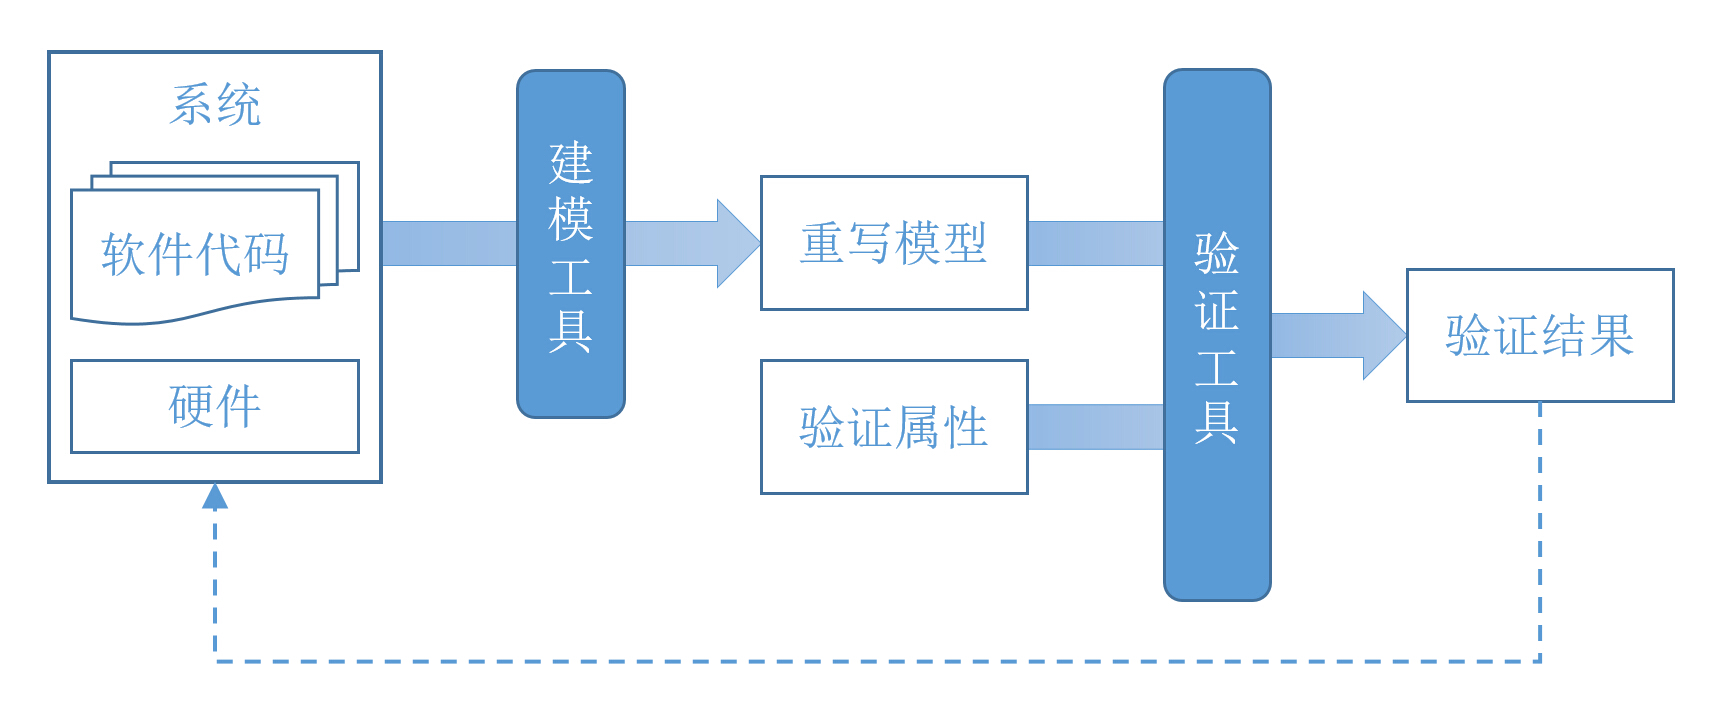
\includegraphics[width=\textwidth]{framework.jpg}
\caption{基于重写模型的形式化建模与验证流程}
\label{f:framework}
\end{figure}

在这个流程中,建模通常是一个抽象的过程。建模过程需要针对用户所关心的系统属性,对系统的某个侧面进行抽象描述。而抽象的层次,则需要建模人员根据经验进行斟酌。如果抽象层次太低,系统模型将包含大量细节,模型行为将更贴近目标系统的行为,验证结果也更有指导意义。然而模型中细节过多可能导致的后果是在验证过程中,验证工具无法处理如此大规模的模型验证。另一方面,如果抽象层次太高,虽然有利于后端验证过程的进行,但由于模型的行为描述太抽象,对应的验证结果可能对目标系统没有太多指导意义。

下面先介绍基于重写模型的系统建模思路,然后针对嵌入式系统所具有的一些特征,介绍如何利用重写模型对这些特征进行建模。

\subsection{建模框架}

\subsubsection{系统状态建模}
\label{sss:state-modeling}

对系统进行建模,首先需要对系统某一时刻的运行状态进行建模。对于基于状态的模型(比如自动机等)来说,系统的状态可以对应为模型的状态,这比较易于理解。而对于基于项表达式和规则的重写模型来说,系统状态则需要通过项表达式来进行建模。

具体地说,在基于重写模型进行系统建模时,我们通过定义函数符号来对我们所关心的系统元素(如变量、状态等)进行“编码”。通过人为地给函数符号及其每一个参数赋予语义,来给每一个项表达式赋予语义。比如在例~\ref{e:river} 中,我们规定函数符号 $\farmer$、$\wolf$、$\lamb$、$\grass$ 各自表示农夫、狼、羊、草当前所处的状态,而它们的第一个参数则表示当前该对象处于河的哪一侧。我们又规定函数符号 $\lhs$ 和 $\rhs$ 分别表示河的左岸和右岸,于是项表达式 $\farmer(\lhs) \comp \lamb(\lhs) \comp \wolf(\rhs) \comp \grass(\lhs)$ 就可以用于表示系统的某个状态,该状态为农夫在左岸、羊在左岸、狼在右岸、草在左岸。又比如在例~\ref{e:clock} 中,我们规定函数符号 $\clock$ 表示一个时钟当前的状态,而它的第一个参数表示该时钟当前的读数。而我们又给 $\s$ 和 $\zero$ 赋予了自然数的语义,于是项表达式 $\clock(\s^3(\zero))$ 就可以表示系统的某个状态,该状态的时钟读数为 3。

需要特别注意的是,项表达式可以对系统中用户自定义的数据类型进行描述。如定义~\ref{d:term} 所示,由于项表达式利用归纳方式进行定义,与函数式编程语言(如 Haskell)中数据类型的定义方式相同,因此可以对诸如结构体、链表、二叉树等自定义数据类型进行建模。

\subsubsection{系统行为建模}
\label{sss:behavior-modeling}

系统行为,可以理解为系统状态的改变方式。对于基于状态的模型来说,连接模型状态之间的变迁,就是模型状态的改变方式。因此对于这些模型来说,系统行为可以利用变迁进行建模。而对于重写模型,系统状态由项表达式来表示,因此作为定义项表达式之间变换关系的重写规则,可以用于建模系统的状态变迁,即系统行为。

具体地说,重写规则的左项表示变迁发生前的系统状态(或部分状态),规则的右项表示变迁发生后的系统状态(或部分状态),而重写规则的条件约束则定义了发生该变迁所需满足的条件。需要注意的是,由于重写规则可以包含变量符号,因此一条重写规则可以描述一种状态变迁\emph{模式},即一类状态变迁,而不仅仅是某条状态变迁。比如在例~\ref{e:river} 中,规则 $\farmer(x)\comp \lamb(x) \ra \farmer(\change(x))\comp\lamb(\change(x))$ 描述的行为是,如果当前状态为农夫和羊在河的同侧$x$,那么下一个状态,农夫和羊将会同处于河的另一侧 $\change(x)$。$x$ 可以是 $\lhs$(左岸),也可以是 $\rhs$(右岸)。又比如在例~\ref{e:clock} 中,规则 $\clock(x) \ra \clock(\add(x,\s(\zero))) \;\Dla\; \lessthan(x,\s^{11}(\zero)) = \true$ 表示,如果当前状态的时钟示数为 $x$,且满足 $x < 11$,那么下一个系统状态\emph{有可能} 为时钟示数显示 $x+1$。注意这里“有可能”的意思是,由于重写的不确定性,该状态的下一个系统状态,根据规则 $\clock(x) \ra \broken$,也有可能为 $\broken$,即表示时钟损坏。

虽然重写规则本身并不对规则两侧的项表达式作任何形式上的约束,但在利用重写模型进行系统建模时,我们通常会在两侧使用“同类型”的项表达式。这指的是,规则两侧的项表达式所建模的系统状态或元素是相同类型的。比如例~\ref{e:clock} 的规则 $\clock(x) \ra \broken$,两侧的项表达式 $\clock(x)$ 和 $\broken$ 所建模的都是系统中时钟的状态。如果存在规则 $\clock(x) \ra x$,左项表示的是时钟的状态,而右项是一个自然数,则该规则从系统行为的角度来看是不合理的。

\subsection{组件层次与并发}
\label{ss:multi-component}

一个嵌入式系统可能由若干个子模块构成,系统的功能需要由各子模块之间协作共同完成;另一方面,与通用计算机不同,嵌入式系统一般用于实现特定功能,它往往作为更上层系统的一部分,与其它嵌入式系统共存。因此,要对嵌入式系统进行建模,则要求模型本身支持组件行为的可组合性及其并发的描述。

首先需要指出,在定义~\ref{d:rewriting} 中,重写对项表达式的影响被位置 $p$ 所约束。也就是说,重写是局部进行的——当我们对某个项表达式应用重写规则进行重写时,被替换的部分不需要是整个项表达式,可以只限定于某个子项表达式。转换成系统建模的视角,这表明,通过重写规则定义的系统行为,不一定改变了整个系统状态,可以只是系统一部分的状态,即系统中某个组件的状态。

基于以上思路,多组件系统的层次结构可以利用项表达式的层次结构(定义~\ref{d:term})进行描述。假设我们用项表达式 $t_1,\ldots,t_n$ 分别对系统中 $n$ 个组件的状态进行建模,那么可以定义一个新的 $n$ 元函数符号 $f^{(n)}$,用项表达式 $f(t_1,\ldots,t_n)$ 来对整个系统状态进行建模。

至于组件行为的组合,得益于重写的局部性,定义在子项表达式上的重写规则,可以自然地应用到整个项表达式上。也就是说,子组件的行为可以在系统中独立进行。比如说,假设我们定义了重写模型 $\cR_i$ 对子组件 $i$ 的行为进行建模。那么 $\cR_i$ 的规则可以被应用于项表达式 $t_i$,表示子组件 $i$ 的状态变化。当子组件 $i$ 被置于整个系统 $f(t_1,\ldots,t_n)$ 中看待时,子组件 $i$ 的局部行为并不受影响,$\cR_i$ 的规则仍然可直接被应用于 $f(t_1,\ldots,t_n)$ 的子项表达式 $t_i$,并且不影响其它子项表达式 $t_j$($j\not=i$)。正如例~\ref{e:river},我们把农民、狼、羊和草各自看作系统中的一个子组件,整个系统的状态由函数符号“$\comp$”将各子组件连接构成。规则 $\farmer(x) \ra \farmer(\change(x))$ 实际上定义了“农民”这个子组件的行为,但它仍然可以被(局部)应用于系统状态 $\farmer(\rhs) \comp \lamb(\rhs) \comp \wolf(\lhs) \comp \grass(\lhs)$,产生新的系统状态 $\farmer(\lhs) \comp \lamb(\rhs) \comp \wolf(\lhs) \comp \grass(\lhs)$,表示农夫独自到了河对岸,而系统中其它子组件不受影响。重写技术的局部性,使组件之间的并发行为在重写模型中得到表达~\cite{DBLP:journals/tcs/Marte-OlietM02}。

\begin{figure}[ht]
\centering
\begin{tikzpicture}
\draw (0,0) rectangle +(2.4,1.6);
\draw (1.2,0.8) node[align=center] {$\cF_1$ \\ $\lb \cR_1,\cS_1,\cE_1\rb$};
\draw [-{Latex}] (1.2,1.6) -- +(0,0.4);
\draw (3,0) rectangle +(2.4,1.6);
\draw (4.2,0.8) node[align=center] {$\cF_2$ \\ $\lb \cR_2,\cS_2,\cE_2\rb$};
\draw [-{Latex}] (4.2,1.6) -- +(0,0.4);
\draw (6.7,0.8) node[align=center] {$\ldots\;\ldots$};
\draw (8,0) rectangle +(2.4,1.6);
\draw (9.2,0.8) node[align=center] {$\cF_n$ \\ $\lb \cR_n,\cS_n,\cE_n\rb$};
\draw [-{Latex}] (9.2,1.6) -- +(0,0.4);

\draw (0,2) rectangle +(10.4,0.8);
\draw (5.2, 2.4) node [align=center] {$\cF_0, \lb\cR_0,\cS_0,\cE_0\rb$};

\draw [dashed] (-0.4,-0.4) rectangle +(11.2,4.6);
\draw (5.2, 3.5) node [align=center] {$\cF=\bigcup^n_{i=0}\cF_i, \lb \cR = \bigcup^n_{i=0}\cR_i, \cS = \bigcup^n_{i=0}\cS_i, \cE = \bigcup^n_{i=0}\cE_i \rb$};
\end{tikzpicture}
\caption{规范化条件重写模型的层次结构}
\label{f:layered-model}
\end{figure}

图~\ref{f:layered-model} 描述了当系统中存在多组件时,利用规范化条件重写模型对系统进行建模的模型层次结构。假定模型 $\lb \cR_i,\cS_i,\cE_i\rb$($1\le i\le n$)是子组件 $i$ 的行为模型。当考虑整个系统时,除了将 $\cR_i$、$\cS_i$、$\cE_i$ 直接叠加(取并集),还需要定义新的词汇表 $\cF_0$ 对系统整体状态进行建模(比如例~\ref{e:river} 的函数符号“$\comp$”),以及定义新的模型 $\lb \cR_0,\cS_0,\cE_0\rb$ 描述各组件之间的交互行为(比如同步、异步通信)。然后整个系统则可以由模型 $\lb \cR,\cS,\cE\rb$ 进行描述,其中 $\cR = \bigcup^n_{i=0}\cR_i$、$\cS = \bigcup^n_{i=0}\cS_i$、$\cE = \bigcup^n_{i=0}\cE_i$。如果系统存在更上层结构,则“递归地”进行以上建模过程。

\subsection{组件交互}

上一小节介绍了组件行为的组合建模,以及各组件局部行为之间的并发。当组件之间存在交互时,需要定义新的模型 $\lb \cR_0,\cS_0,\cE_0\rb$ 用于描述组件之间的交互行为。下面分别从同步和异步两种方式来介绍重写模型如何对组件之间的交互行为进行建模。


\subsubsection{同步}
\label{ss:sync}

组件之间的同步通信,实际上是指若干组件在满足某条件时同时发生状态改变。从重写模型的角度来说,这需要重写规则同时应用于各组件对应的子项表达式。因此,描述同步行为的重写规则应该定义在描述整个系统的项表达式上,即包含 $f\in\cF_0$ 的项表达式。该规则的左项不应该仅仅包含某个子组件对应的子项表达式,而应该包含该同步行为涉及的所有组件对应的多个子项表达式。比如在例~\ref{e:river} 中,重写规则 $\farmer(x)\comp \wolf(x) \ra \farmer(\change(x))\comp\wolf(\change(x))$ 是一条描述同步行为的规则。规则的左项包含了组件“农民”和“狼”,只有满足农民和狼的位置相同(都为 $x$)这一条件,该同步行为才能发生。产生的状态变化是:农民和狼同时来到了 $x$ 的另一侧 $\change(x)$。

举个例子,比如我们希望描述一个具有两个时钟的系统,我们定义二元函数符号 $f^{(2)}$ 来建模整个系统的状态,它的两个参数都是例~\ref{e:clock} 中定义的 $\clock$,分别代表两个时钟当前的状态。因此 $f(\clock(\zero),\clock(\s(\zero)))$ 表示当前系统状态为:时钟1的示数为 0,时钟 2 的示数为 1。如果我们希望两个时钟同步运行,那么我们不能使用例~\ref{e:clock} 中给单个时钟定义的重写规则,它们会产生重写序列:
\begin{eqnarray}
 f(\clock(\s^0(\zero)),\clock(\s^0(\zero)))  
 & \ra & f(\clock(\s^1(\zero)),\clock(\s^0(\zero))) \nonumber \\
 & \lrps{}{} & f(\clock(\s^2(\zero)),\clock(\s^0(\zero))) \nonumber \\
 & \lrps{}{} & f(\clock(\s^2(\zero)),\clock(\s^1(\zero))) \mbox{。} \nonumber
\end{eqnarray}
以上序列表明两个时钟是各自并发运行的,之间没有任何关系。我们需要定义以下同步规则\footnote{注意这里为了方便理解,该规则省略了应满足的约束条件 $x<11$。}
\begin{eqnarray}
 f(\clock(x),\clock(x)) & \ra & 
 f(\clock(\add(x,\s^1(\zero))),\clock(\add(x,\s^1(\zero)))) \nonumber
 \end{eqnarray}
描述满足我们需求的同步行为:当系统中的两个时钟示数相同(都为 $x$)时,两个时钟的示数同时加 1。于是有以下重写序列,描述了系统中两个时钟同步运行:
\begin{eqnarray}
 f(\clock(\s^0(\zero)),\clock(\s^0(\zero)))  
 & \ra & f(\clock(\s^1(\zero)),\clock(\s^1(\zero))) \nonumber \\
 & \lrps{}{} & f(\clock(\s^2(\zero)),\clock(\s^2(\zero))) \nonumber \\
 & \lrps{}{} & f(\clock(\s^3(\zero)),\clock(\s^3(\zero))) \mbox{。} \nonumber
\end{eqnarray}

\subsubsection{异步}
\label{ss:async}

异步事件触发的行为可以抽象地拆解成两个行为:组件 1 触发事件 A,事件 A 使组件 2 的状态发生变化。如果将事件 A 看作系统中的一个子组件,则这两个行为可以分别看作两个同步行为。在对异步行为进行建模时,我们采取这种方式把异步行为拆解成两个同步行为进行建模。

下面举个例子说明。假设组件 1 的状态可以从 $a$ 变成 $b$,从 $b$ 变成 $c$,从 $c$ 变成 $d$;当它从状态 $b$ 变成状态 $c$ 时,同时会给系统中的组件 2 发送一个消息 $m$。假设组件 2 在状态 $e$ 会等待从组件 1 发送过来的消息 $m$;收到消息后状态会变成 $g$。那么我们将组件 1 和组件 2 之间用于传输消息 $m$ 的信道也作为系统的一个组件进行考虑。定义三元函数符号 $f^{(3)}$ 用于建模系统状态,它的第一个参数表示组件 1 的状态,第二个参数表示信道的状态,第三个参数表示组件 2 的状态。于是我们可以用以下规则来对上述异步行为进行描述:
\begin{eqnarray}
 a & \ra_1 & b \nonumber \\
 f(b,x,y) & \ra_2 & f(c,m,y) \nonumber \\
 c & \ra_3 & d \nonumber \\
 f(x,m,e) & \ra_4 & f(x,\myempty,g) \;\mbox{,} \nonumber
\end{eqnarray}
其中常数 $\myempty$ 表示信道中无消息。 规则 2 是组件 1 和信道组件的同步行为,它表示“组件 1 的状态从 $b$ 变成 $c$”这个动作必须和“信道中有消息 $m$ 出现”这个动作同时发生,且注意该同步行为不涉及组件 2——其状态 $y$ 不发生改变。而规则 4 则是信道组件和组件 2 的同步行为,它表示“信道中的消息 $m$ 消失”这个动作必须与“组件 2 的状态从 $e$ 变成 $g$”这个动作同时发生。规则 2 和规则 4 是典型的异步行为建模规则。由上述规则可以产生如下重写序列:
\begin{eqnarray}
& & f(a,\myempty,e)  \ra  f(b,\myempty,e) 
  \ra f(c,m,e) \ra f(d,m,e)  \ra f(d,\myempty,g) \;\mbox{。} \nonumber
\end{eqnarray}
该序列表明,组件 1 向组件 2 发出消息 $m$ 后,不需等待组件 2 的响应,即可继续运行(从状态 $c$ 变成状态 $d$)。需要注意的是,状态 $b$ 与 $g$ 可以进一步细化为与消息 $m$ 有关的项表达式,如 $b=b'(m)$、$g=g'(m)$,表示组件 1 向组件 2 传递信息。 


\subsection{软硬件行为}
\label{ss:hw-sw}

嵌入式系统通常由软硬件混合构成,而软件与硬件的行为差异在于,硬件行为通常具有并发性,而软件代码通常以顺序方式执行。从建模的角度对组件的顺序行为与并行行为进行考虑,它们可以进一步被抽象成两类行为——确定性行为与不确定性行为,分别对应于规范化条件重写模型 $\RSE$ 的规则集 $\cS$ 与 $\cR$。

对组件的局部行为,若是顺序执行的(例如不涉及共享变量访问的软件代码),则将其建模为局部确定性行为,即建模为 $\cS_i$ 的重写规则;若该行为具有不确定性(例如硬件模块随时可能发生物理失效),则将其建模为局部不确定性行为,即通过 $\cR_i$ 的重写规则进行建模。对组件间的交互行为,考虑到它可能对系统中其它行为产生影响(例如对共享变量进行写操作可能影响其它线程对该变量的读操作),因此将其建模为全局的不确定性行为,即描述为 $\cR_0$ 的重写规则。

\begin{figure}[ht]
\centering
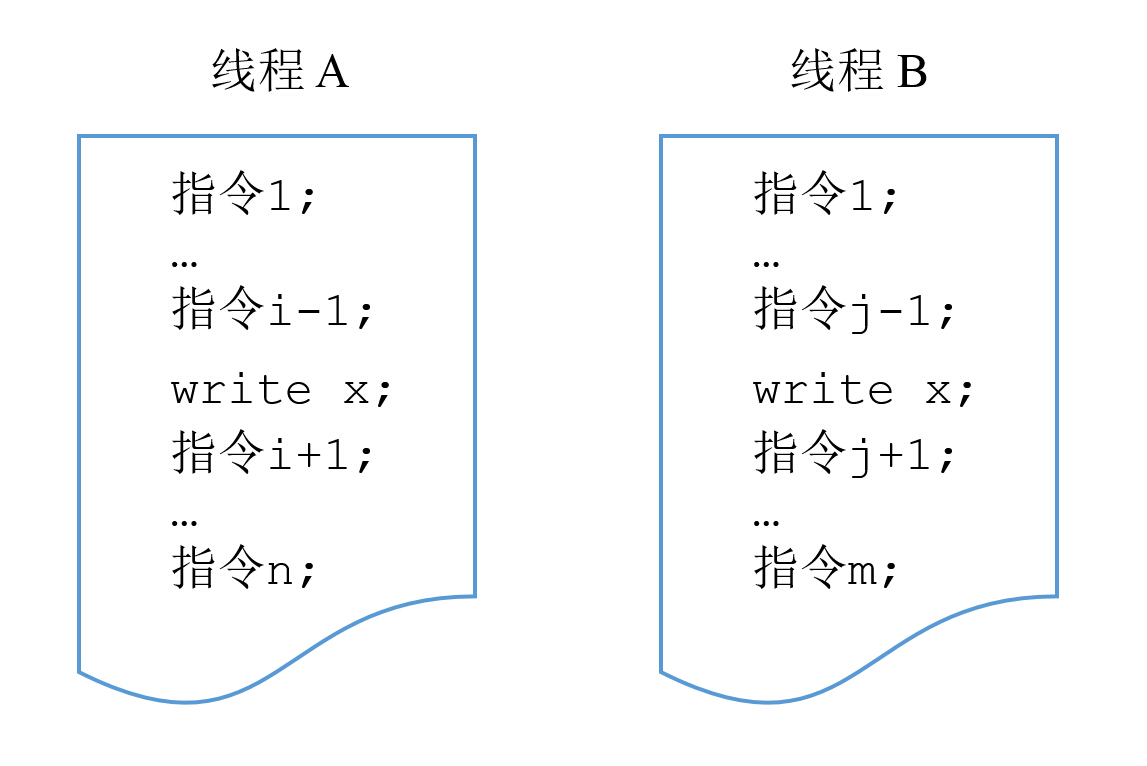
\includegraphics[width=0.7\textwidth]{concur.jpg}
\caption{两个线程的并发}
\label{f:concur}
\end{figure}

如图~\ref{f:concur} 的例子,假设变量 x 是全局变量,线程 A 的指令 i 和线程 B 的指令 j 都对 x 进行写操作,因此这两条指令被调度运行的先后次序将对整个系统的运行结果产生影响,它们应当被建模成 $\cR_0$ 中的全局不确定性规则。假设线程 A 的其它指令以及线程 B 的其它指令都与变量 x 无关,虽然这些指令相互之间并发运行,但实际上系统对这些指令的调度并不会影响运行结果,因此它们可被建模成 $\cS_i$ 的局部确定性规则。

从模型组合的角度来看,不同组件的局部确定性行为 $\cS_i$ 作用于项表达式的不同位置,因此这些行为组合得到的系统行为模型 $\cS$ 具有终止性与合流性~\cite{DBLP:journals/jacm/Huet80},满足规范化条件重写模型 $\RSE$ 的要求。

根据规范化重写的定义(定义~\ref{d:normalrewriting}),$\cS$ 规则的应用是附属于 $\cR$ 规则的,以上建模策略让系统中行为的重要程度在规范化重写模型中有所体现。另一方面,根据定义~\ref{d:normalrewriting},应用 $\cR$ 规则前后都需要对整个项表达式应用 $\cS$ 规则进行规范化,这就保证了规范化重写序列与系统状态变迁路径的对应性。同时,在这一建模策略下,由于 $\cS$ 规则对应的行为被“嵌入”到 $\cR$ 规则对应的行为中,相当于若干行为被抽象成单一行为,这使得系统的状态空间数得以减少\footnote{这意味着被抽象的中间状态必须与验证属性无关。},为后端的验证过程提供了便利。


\subsection{组件的动态结构}
\label{ss:dynamic-component}

在嵌入式系统中,存在组件结构的动态行为。比如在事件响应系统中,接收到一个事件请求后,系统可能创建一个新线程对该事件进行处理;又比如在无线传感网络中,因为主观连接需求或者客观的通信信号问题,网络中的节点拓扑通常会产生变化。这些行为都涉及到组件结构的改变。
这就对建模模型提出了两个问题:如何对这种组件结构变化进行建模?如何对新增的组件行为进行建模?

首先是对组件结构变化的建模方式。由于项表达式描述的不仅仅是系统中某些变量的状态,而是整个系统的状态,其中包括系统的结构信息。在第~\ref{ss:multi-component} 小节中提到,系统组件的数量由函数符号的元数进行描述。如果系统中组件数量可变,那么我们需要函数符号的元数可变——这违背了词汇表 $\cF$ 的定义。然而,得益于规范化重写模型丰富的表达能力,我们可以利用等价模型 $\cE$ 来模拟元数可变的函数符号。实际上,解决思路早已在例~\ref{e:river} 中给出——定义二元(中缀)函数符号“$\comp$”。如果它具有结合律,即以下等价规则属于 $\cE$,
\begin{eqnarray}
 (x\comp y) \comp z & \sim & x \comp (y\comp z)\;\; , \nonumber
\end{eqnarray}
那么由“$\comp$”构成的项表达式中的括号可以省略。它定义了一个列表结构,列表中的元素数量可变。例如 $a\comp b$、$a\comp b\comp c\comp d$、$a\comp b\comp c\comp d\comp e$ 都是列表。如果函数符号“$\comp$”同时还具有交换律,即以下等价规则属于 $\cE$,
\begin{eqnarray}
 x\comp y & \sim & y\comp x\;\; , \nonumber
\end{eqnarray}
那么由“$\comp$”构成的项表达式中,不仅括号可以省略,而且元素之间的顺序变得无关重要。它定义了一个多重集合结构,多重集合中的元素数量可变,且元素无序。例如 $a\comp a\comp c\comp d$ 和 $a\comp d\comp c\comp a$ 都是多重集合,且 $(a\comp a\comp c\comp d) =_{\cE} (a\comp d\comp c\comp a)$。下面假设“$\comp$”同时具有交换律和结合律。

基于这种结构可变的模型,改变结构的行为可以被建模成对应的改变项表达式结构的重写规则。例如要描述以下行为:线程 $f$ 在状态 $a$ 创建一个新线程 $g$,$g$ 的初始状态为 $a'$,而线程 $f$ 在创建 $g$ 以后进入状态 $b$。那么我们可以用以下重写规则:
\begin{eqnarray}
f(a) & \ra & f(b) \comp g(a') \nonumber
\end{eqnarray}
来描述线程 $g$ 的创建过程。又比如在例~\ref{e:river} 中,我们可以用以下规则:
\begin{eqnarray}
\wolf(x)\comp\lamb(x) & \ra & \wolf(x) \nonumber
\end{eqnarray}
描述狼把在同侧的羊吃掉的行为。这也是一种系统组件结构发生变化的行为。

在对“产生新组件”这一行为进行建模后,还需要对新组件本身的行为进行建模。由于新组件的行为是可预知的(比如处理某类事件的方式),因此描述新组件行为的重写规则只需如其它行为一样,定义在规则集 $\cS$ 或 $\cR$ 中即可。

在这里我们可以看到基于重写模型建模的一大优点:基于项表达式的状态建模,可以描述系统结构的变化,使建模人员不需要对动态产生的新组件数量上限进行假设。

\subsection{实时性}
\label{ss:realtime-modeling}

许多嵌入式系统的正确性不仅要求满足逻辑正确性,还需要满足某些时间约束,这类系统称之为\emph{实时系统}。对于实时系统的建模,要求模型中支持对“时间”的建模。针对重写模型,我们在系统的项表达式中,增加一个用于描述时间的子项表达式,例如项表达式
\begin{eqnarray}
& & f(t_1,\ldots,t_n,\; time) \nonumber
\end{eqnarray}
中,$f^{(n+1)}$ 的最后一个参数。而位于 $time$ 位置的子项表达式可以采用自然数集(如例~\ref{e:nat})表示离散的时间,也可以采用非负实数集~\cite{DBLP:journals/tcs/GoguenM92} 表示连续的时间,这取决于建模人员对模型精确度的要求,也取决于验证工具的验证能力。

需要注意的是,由于我们将“时间”作为组件在模型中进行描述,因此系统中所有需要耗时的行为都将被建模成同步行为,需要与“时间”组件进行同步。例如下列规则:
\begin{eqnarray}
f(a,\; x_{time}) & \ra & f(b,\; x_{time}+1) \nonumber
\end{eqnarray}
描述了系统从状态 $a$ 变成状态 $b$ 的行为,这一行为需要耗时 1 个时间单位。

\section{支持工具集}
\label{s:tool}

本小节将基于语义映射的方式,将上述建模框架在工具集 Maude 中予以实现。

\subsection{Maude}

\emph{Maude}~\cite{DBLP:journals/tcs/ClavelDELMMQ02} 是一种基于重写逻辑~\cite{DBLP:journals/jlp/Meseguer12} 的语言和工具,它能支持形式化建模和对模型的分析验证。

\subsubsection{建模}
Maude 将系统建模成为\emph{模块}(module)。一个模块相当于一个\emph{重写逻辑模型}(rewrite theory) 
$\mathcal{R^L} = \lb\Sigma,\mathit{A},\mathit{E} , \mathit{R}\rb$,其中:
\begin{itemize}
\item $\Sigma$ 是一个带类型的词汇表。它包括函数符号、\emph{类型}\footnote{注意这里应指\emph{类别},与“类型”有所区别。为了便于读者理解,本文称之为“类型”。}(sort)和\emph{子类型}(subsort)的声明。 函数符号允许使用中缀记法、前缀记法、后缀记法或混合记法,利用下划线“\verb|_|” 表示参数的位置。项表达式的定义与重写模型相同。
\item $\lb\Sigma, \mathit{E}\cup\mathit{A}\rb$ 是一个\emph{带成员关系的等词逻辑理论}~\cite{DBLP:journals/tcs/BouhoulaJM00}(membership equational logic theory)。其中,$\mathit{E}$ 是条件等式(conditional equation)和成员关系规则的集合,
$\mathit{A}$ 是一个性质集合,比如交换律、结合律等。
\item $\mathit{R}$ 是一个\emph{带标签的条件重写规则} 集合。它描述了系统的单步状态变迁。每一条规则的形式为 $[l]~:~t\rightarrow t'\mbox{ \textbf{if}
  }\bigwedge^n_{j=1}cond_j$,其中 $cond_j$ 是形如 $u_j=v_j$ 的约束条件,$l$ 是该规则的标签,$t,t',u_j,v_j$ 都是项表达式。该规则的语义与条件重写规则(定义~\ref{d:crule})的语义相同。
\end{itemize}

Maude 还支持面向对象风格的建模。类声明
\begin{eqnarray}
& & \texttt{class }C\texttt{ |
}att_1\texttt{:}s_1\texttt{,}\ldots\texttt{,}att_n\texttt{:}s_n \nonumber
\end{eqnarray}
定义了一个新类,类名为 $C$,它包含类属性 $att_1,\ldots,att_n$,它们分别具有类型 $s_1,\ldots,s_n$。类 $C$ 的一个\emph{对象}(或称“\emph{实例}”)表示为项表达式
\begin{eqnarray}
\texttt{< } O\texttt{:} C \texttt{ | }
att_1\texttt{:}val_1\texttt{,} \ldots
\texttt{,}att_n\texttt{:}val_n\texttt{ >} \;\mbox{。} \nonumber
\end{eqnarray}
其中,$O$ 是该对象的\emph{标识}(identifier),具有类型 \verb|Oid|;
$val_i$ 是属性 $att_i$ 的值。所有类的对象都具有类型 \verb|Object|。重写规则可以针对某个类的项表达式进行定义。\emph{子类}(subclass)可以继承其父类的所有类属性以及相关的重写规则。

\emph{Real-Time Maude}~\cite{DBLP:journals/lisp/OlveczkyM07} 是 Maude 的一个扩展,它同时给 Maude 语言和工具集增加了新功能。它主要的目的是让 Maude 可以支持实时系统的建模和分析验证。在Maude的基础上,Real-Time Maude 内置了一个名为“\verb|Time|”的描述时间的模块。在 Maude 模块的基础上,Real-Time Maude 在集合 $\mathit{R}$ 中加入了\emph{带标签的单元计时规则}(labeled tick rule)。单元计时规则具有以下形式
\begin{eqnarray}
& & [l]~:~\{s\}\rightarrow\{s'\} \mbox{\textbf{ in time}
  }r\mbox{ \textbf{if} }cond \;\; , \nonumber
\end{eqnarray} 
用于描述系统的时间行为。它表示当条件 $cond$ 满足时,系统从状态 $s$ 变成目标状态 $s'$,(全局)时间往前推移 $r$ 个时间单位。为了区别于单元计时规则,$\mathit{R}$ 中原来的不涉及时间的重写规则,称作\emph{瞬时规则}(instantaneous rule),应用该规则时(全局)时间保持不变。

需要注意的是,Maude 面向对象风格的模型以及其扩展 Real-Time Maude 都只是一种语法封装,它们的底层仍基于重写逻辑模型 $\mathcal{R^L}$ 和重写逻辑。 

\subsubsection{模型分析及形式化验证}
给定一个重写逻辑模型,Maude 和 Real-Time Maude 给用户提供了许多配套工具对模型进行分析。例如,\verb|rewrite| 指令可以符号化地、抽象地执行目标模型,在模型的层次上对系统进行仿真;给定一个初始状态(用项表达式表示),\verb|search| 指令可以搜索所有可达的状态,从中判断是否存在满足指定性质的状态;Maude 配套的\emph{交互式定理证明器}~\cite{DBLP:journals/jucs/ClavelPR06}(Inductive Theorem Prover,ITP)可以通过交互式的方法,用于证明模型具有的等词逻辑性质。

在本文中,我们更关心的是 Real-Time Maude 配套的形式化验证工具——\emph{LTL 模型检测器}~\cite{DBLP:journals/entcs/EkerMS02}(LTL model checker)。它可以检查是否模型中的\emph{任意} 一条行为路径都满足给定的时序逻辑公式。\emph{状态命题}(state proposition)被定义为具有类型 \verb|Prop| 的项表达式。它们的语义由集合 $\mathit{E}$ 中以下形式的条件等式进行规定:
\begin{eqnarray}
\texttt{ceq
} \mathit{statePattern} \texttt{ |= } \mathit{prop} \texttt{ = } b
\texttt{ if } cond\;\; , \nonumber
\end{eqnarray}
其中,$b$ 是具有类型 \verb|Bool| 的项表达式。该条件等式表示,当 $cond$ 成立且当前状态的项表达式是 $\mathit{statePattern}$ 的实例时, $\mathit{prop}$ 的值等于 $b$。所有这种形式的条件等式共同定义了命题 $\mathit{prop}$ 成立的条件:命题 $\mathit{prop}$ 在状态 $s$ 成立,当且仅当 $s$ 满足 $s \texttt{ |= } \mathit{prop}$ 等于 \verb|true|。\emph{时序逻辑公式}~\cite{DBLP:books/daglib/0077033}(temporal logic formula)由状态命题和时序逻辑操作符(operator)构成。时序逻辑操作符包括但不限于 \verb|~|(非)、\verb|\/|(或)、\verb|[]|(“总是”)、\verb|<>|(“最终”)、\verb|U|(“直到”)。 Real-Time Maude 支持\emph{时控的}(timed)和\emph{非时控的}(untimed)LTL 模型检测。本文的案例将会用到非时控的 LTL 模型检测命令
\begin{eqnarray}
  \texttt{(mc } s \texttt{ |=u } \Phi \texttt{ .)} \nonumber
\end{eqnarray}
该命令检查的是,给定初始状态 $s$,从 $s$ 开始的所有行为序列是否\emph{在所有时刻} 都满足时序逻辑公式 $\Phi$。


\subsection{建模框架实现} 
\label{ss:method-impl}

如果将重写逻辑模型 $\mathcal{R^L} = \lb \Sigma, A, E, R\rb$ 的 $\Sigma$、$A$、$E$、$R$ 分别与规范化条件重写模型 $\RSE = \lb \cR,\cS,\cE\rb$ 的 $\cF$、$\cE$、$\cS$、$\cR$ 对应起来,两者存在许多相似之处,然而它们的主要区别在于:
\begin{enumerate}[(i)]
\item 重写逻辑模型 $\mathcal{R^L}$ 的性质集合 $A$ 只支持交换律、结合律、单位元性质(identity)和幂等性(idempotency),而规范化条件重写模型 $\RSE$ 的等价模型 $\cE$ 支持一般化的等式规则,覆盖了 $A$ 的支持范围;
\item 重写逻辑模型 $\mathcal{R^L}$ 的重写过程基于类重写~\cite{lankford77b},即重写规则应用的对象是项表达式关于 $E$ 的等价类,而规范化条件重写(定义~\ref{d:cnormalrewriting})基于规范化过程,即重写规则应用的对象是项表达式关于 $\cS$ 的范式;
\item 重写逻辑模型 $\mathcal{R^L}$ 带类型信息,而规范化条件重写模型 $\RSE$ 不带类型信息。
\end{enumerate}

区别 (ii) 是两者在理论模型上的区别。然而,Clavel 等人在文献~\inlinecite{DBLP:journals/tcs/ClavelDELMMQ02} 中指出,Maude 在具体实现时,为了保证工具效率,采取了与规范化重写相似的重写策略。
%——将 $E$ 中的条件等式看作有向规则,并利用 $E$ 对项表达式进行规范化。

\begin{algorithm}[ht] 
    \KwIn{规范化条件重写模型四元组 $\cF$, $\cE$, $\cS$, $\cR$}
    \KwOut{重写逻辑模型四元组 $\Sigma$, $A$, $E$, $R$}

    $\Sigma = \cF$\;
    $R = \cR$\;
    $A = \emptyset$\;

    \ForEach{$e \in \cE$}{
        \If{$e$ 表示交换律、结合律、单位元性质或幂等性}{
            $A = A \cup \{e\}$\;    
        }
    }

    $\cE' = \cE \setminus A$\;
    bool $exist = false$\;

    \tcp{$directed(\cE')$ 计算 $\cE'$ 中等式有向化产生的所有可能的重写规则集}
    \ForEach{$\vec{\cE'} \in directed(\cE')$}{
        \If{模重写模型 $(\vec{\cE'}\cup\cS)_A$ 是终止且合流的 }{
            $exist = true$\;
            break \;    
        }
    }

    \uIf{ $exist = true$ }{
        $E = \vec{\cE'} \cup \cS$\;
    } \Else {
        转换失败\;
    }
\caption{规范化条件重写模型转换成重写逻辑模型}
\label{alg:convert}
\end{algorithm}

因此,本文提出算法~\ref{alg:convert},将(部分)规范化条件重写模型转换为重写逻辑模型。转换的关键点在于:重写逻辑模型的集合 $A$ 所支持的(等式)性质不及规范化条件重写模型的集合 $\cE$ 一般化,因此对于 $\cE$ 中不被支持的等式规则,需要将其有向化,转换成重写规则放入集合 $E$。所以该算法转换成功与否的关键,就在于有向化后的规则集 $\vec{\cE'}$ 能否满足重写逻辑对集合 $E$ 的要求,即必须是终止且合流的。

基于算法~\ref{alg:convert},我们将第~\ref{s:modeling} 小节提出的建模方法在 Maude 中予以实现,并通过两个真实应用案例(第~\ref{s:TO} 小节和第~\ref{s:RMS} 小节),验证它的可行性。 



\section{应用案例:铁路机车节能优化控制系统}
\label{s:TO}

铁路机车节能优化控制系统~\cite{DBLP:journals/tc/HuangDYS16}(以下简称“优化控制系统”)是由清华大学软件学院智能交通实验室与中车信息技术有限公司合作开发的一套铁路机车智能巡航控制与节能产品,用以辅助司机通过自动控制机车来最大限度降低机车的能耗。该系统对机车进行控制的过程中涉及到自动控制与司机手动控制状态的转换。本小节基于第~\ref{s:modeling} 小节提出的建模方法,利用 Maude 工具对该系统的状态转换逻辑进行建模和形式化验证。通过建模过程和验证方法的应用,我们定位了系统中的若干缺陷,并与开发人员进行了确认,帮助开发人员进行修复。

\subsection{背景介绍}

\begin{figure}[ht]
\centering
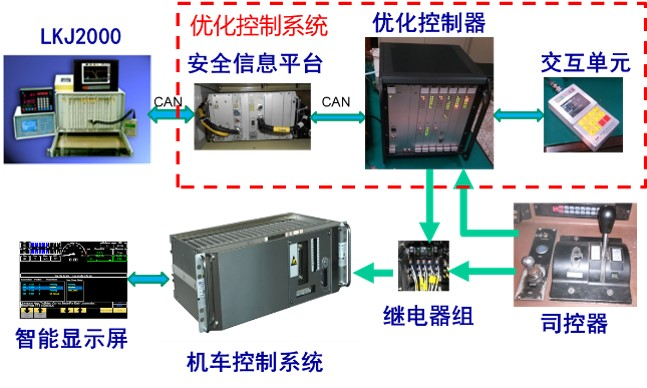
\includegraphics[width=\textwidth]{TO-system.jpg}
\caption{铁路机车节能优化控制系统}
\label{f:TO-system}
\end{figure}

优化控制系统的组成及其涉及到的周边部件如图~\ref{f:TO-system} 所示。LKJ2000 负责向优化控制系统提供铁路线路信息以及实时信息(如信号灯、是否限速等)。在手动控制状态下,机车驾驶员通过司控器进行机车的档位控制。继电器组和机车控制系统对机车进行物理控制。智能显示屏显示机车的实时状态。而优化控制系统本身主要由三部分构成。安全信息平台负责处理从 LKJ2000 接收的数据,向优化控制器提供必要的数据。优化控制器是整个系统的核心,负责列车控制逻辑和控制策略的计算。交互单元则是驾驶员与优化控制器的交互媒介。

机车在运行过程中分为自动控制和手动控制两种状态。机车自动控制时,优化控制器基于离线计算的控制策略,结合在线根据机车状态、线路信息和实时信息计算得到的调整策略,对机车进行控制。当机车处于手动控制状态时,由驾驶员通过司控器对机车进行控制。自动控制状态和手动控制状态之间的转换,可以由驾驶员主动发起,也可能由于机车的状态或铁路的实时信息满足一定条件,从而触发自动和手动控制状态的转换。

机车控制状态的转换由优化控制器负责完成。优化控制器综合从安全信息平台接收的数据、从交互单元获取的操作数据、以及司控器的档位数据,根据业务逻辑计算当前的控制策略(包括是否自动控制、控制档位等)。控制状态转换的逻辑基于事件处理机制。也就是说,优化控制器把安全信息平台向其发送的数据到达看作一个事件,把驾驶员通过交互单元进行的操作也看作一个事件,驾驶员通过司控器调整档位也被当作一个事件。优化控制器对这些外部事件进行处理,产生一个事件(数据帧)发送给继电器组,通知继电器组当前应采取的控制状态及控制档位。图~\ref{f:auto2manual} 是一个从自动控制状态转换成手动控制状态的流程示例。

\begin{figure}[ht]
\centering
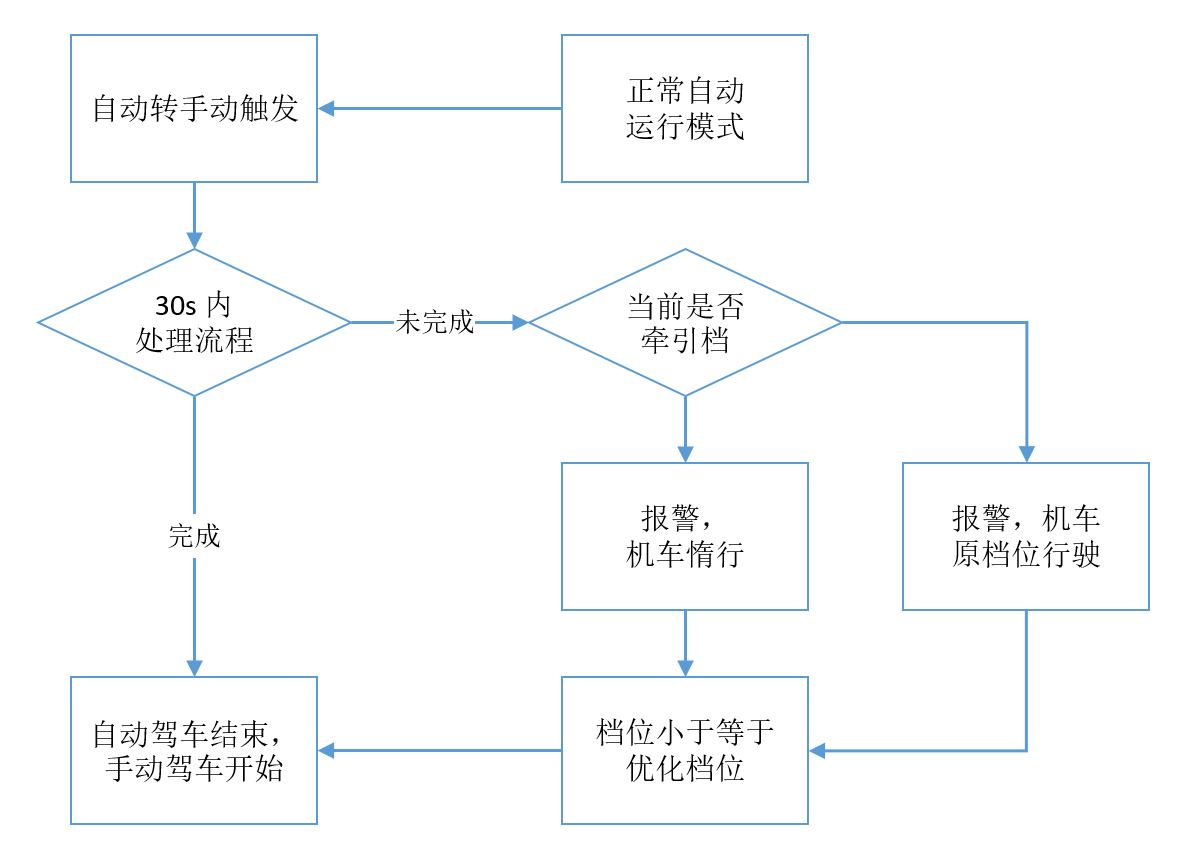
\includegraphics[width=0.9\textwidth]{auto2manual.jpg}
\caption{自动控制到手动控制的转换流程示例}
\label{f:auto2manual}
\end{figure}

优化控制器内部由若干独立模块组成,各模块拥有独立的处理器,且以多线程的方式工作。模块之间的交互也通过事件处理机制完成。因此整个优化控制器,乃至整个优化控制系统,是一个高度并发的分布式系统。系统是否对每一个事件都进行了正确的响应,事件处理的正确性是否受到并发影响,是开发人员及用户迫切关心的问题。本小节主要关心涉及机车控制状态转换的事件处理。


\subsection{系统描述}

\begin{figure}
\centering
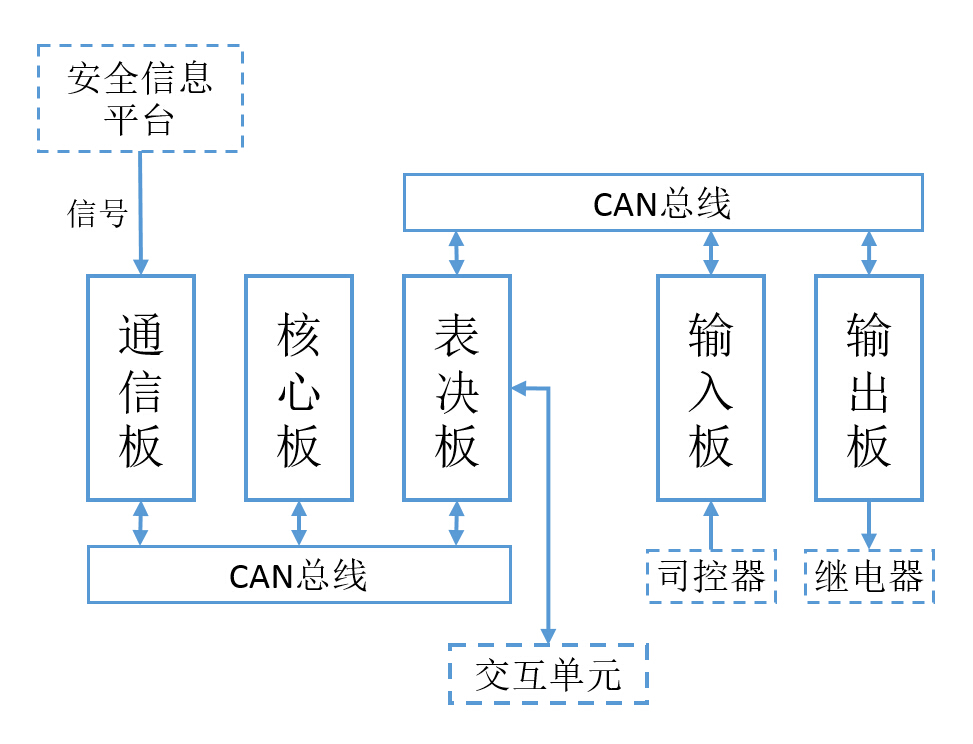
\includegraphics[width=0.7\textwidth]{TO-module.jpg}
\caption{优化控制器内部结构}
\label{f:TO-module}
\end{figure}

优化控制器的内部结构如图~\ref{f:TO-module} 所示,主要由通信板、核心板、表决板、输入输出板以及连接各板卡的总线组成。输入板的功能是将司控器的档位信息发送给表决板。输出板的功能是将表决板的计算结果(控制状态和档位信息)发送到继电器。通信板从安全信息平台接收线路信息以及实时信息,经处理后转发到核心板。核心板接收来自通信板的线路信息和实时信息,根据优化算法计算优化控制策略。然后核心板将优化计算结果发送至表决板。表决板综合考虑来自核心板的优化控制策略、通过交互单元获得的用户操作信息、以及来自输入板的档位信息,根据业务逻辑产生机车的控制策略(自动或手动控制、档位信息等),发送到输出板。

每一块板卡都维护了一个线程池,板卡的每一个端口都有一个单独的线程负责监听。当有新消息帧到来时,负责监听的线程根据该消息帧的类型,创建一个新线程对其进行处理,然后该监听线程继续监听端口消息。被创建的新线程根据自身业务逻辑对该消息帧进行相应的操作,对其计算、转发、触发一个业务流程、或再创建另一个线程等,执行完毕后线程释放。板卡的业务逻辑由多个线程协作共同完成。线程的调度由板上的操作系统完成。


\subsection{系统建模}

我们选择将优化控制系统中的通信板、核心板、表决板、输入输出板以及连接各板卡之间的总线进行建模,并且为安全信息平台和交互单元建立简单的模型,描述它们与优化控制系统之间的交互。

对该系统建模的难点在于:
\begin{enumerate}  
\item 对复杂的数据结构及其存储进行建模。系统由 C 语言实现,代码量巨大,涉及的数据类型复杂,频繁使用各种结构体类型。这要求对数据类型进行建模,且对相应的存储结构(内存)也进行建模。
\item 对板卡间的通信进行建模。
\item 对线程调度进行建模。线程调度由板载操作系统负责,在建模过程中需要考虑线程调度的影响。
\item 对线程以及线程的创建释放进行建模。线程的行为是该系统进行事件处理及实现业务逻辑的关键行为,需要对其进行较准确的刻画。
\end{enumerate}

下面就以上关键点,结合第~\ref{s:modeling} 小节提出的建模方法与第~\ref{ss:method-impl} 小节定义的规范化条件重写模型与 Maude 模型之间的语义映射,对该系统的建模过程进行介绍。

\subsubsection{复杂数据类型及内存}

在第~\ref{sss:state-modeling} 小节已经提到,得益于项表达式的归纳结构,我们可以利用它定义非常复杂的数据类型。同时又得益于 Maude 语言提供的灵活语法,复杂数据结构得以直观地表示。例如我们用 Maude 类型 \verb|RtCore| 对 C 结构体类型 RtCore 进行建模, \verb|RtCore| 的定义如下:
\begin{verbatim}
  sort RtCore .
  op `(rt-gear:_`,rt-enable-status:_`) 
       : Nat Nat -> RtCore [ctor] .
\end{verbatim}
第 1 行用 \verb|sort| 关键字声明了一种新类型。其余两行用 \verb|op| 关键字声明了一个新的函数符号 \verb|(rt-gear:_,rt-enable-status:_)|,它的两个参数分别为 \verb|Nat|(自然数)类型和 \verb|Nat| 类型,返回类型为 \verb|RtCore|。两个下划线“\verb|_|”的位置为该函数符号的两个参数位置。于是项表达式 \verb|(rt-gear:3,rt-enable-status:0)| 表示一个类型为 \verb|RtCore| 的结构体数据,它的 rt-gear 域为 3,rt-enable-status 域为 0。

结构体类型也可以进行嵌套,比如以下表示结构体类型 RtVote 的类型 \verb|RtVote|:
\begin{verbatim}
  sort RtVote .
  op `(rt-core:_`,rt-control-status:_`) 
       : RtCore ControlStatus -> RtVote [ctor] .
\end{verbatim}
它的第一个参数类型为 \verb|RtCore|,是一个表示结构体的项表达式类型。

除了结构体,其它复合类型如第~\ref{ss:dynamic-component} 小节提到的列表和多重集,都可以在 Maude 中进行建模。

针对内存,我们可以用类型 \verb|Pair| 来对内存单元进行建模:
\begin{verbatim}
  op `(_->_`) : Variable Value -> Pair [ctor] .
\end{verbatim}
即 \verb|Pair| 类型的表达式由一个 \verb|Variable| 类型的“变量”表达式与一个 \verb|Value| 类型的“值”表达式组成。\verb|Value| 类型包括 Maude 内置的自然数 \verb|Nat| 类型、布尔 \verb|Bool| 类型以及我们自定义的各种数据结构类型。而内存则是由 \verb|Pair| 类型表达式组成的一个多重集,由连接符“\verb|,|”进行连接。例如项表达式
\begin{verbatim}
  ('x -> 3), ('y -> true)
\end{verbatim}
是一个描述内存状态的项表达式,表示变量 x 值为 3,变量 y 值为 true。

\subsubsection{板卡通信}

为了简化模型,我们假设板卡之间的通信是定向的,即发送时需要指定目标板卡的目标端口。于是我们使用 \verb|Msg| 类型来建模这样一条单向发送通道:
\begin{verbatim}
  op `[==>_:_|_`] : Oid PortType MaybeFrame -> Msg .
\end{verbatim}
其中,\verb|Oid| 类型的参数指定目标板卡,\verb|PortType| 类型的参数指定目标端口,第三个参数是发送的消息帧。而且我们假定这样的发送通道缓冲区大小为 1,每次只能发送一个消息帧。通道被占时会对发送产生阻塞。例如以下表达式
\begin{verbatim}
  [==> VOTE-DES : PORT-CANINOUT 
    | some (gear: 3 ,auto-or-manual: 1) ]
\end{verbatim}
表示通道中包含向 \verb|VOTE-DES|(表决板)的 \verb|PORT-CANINOUT| 端口发送的消息帧,该帧包含档位数据及控制状态数据。

消息的发送与接收行为,则分别可以建模成该通道与发送方以及接收方的同步行为,如第~\ref{ss:sync} 小节及第~\ref{ss:async} 小节所述。 

\subsubsection{线程调度}

由于板卡上线程的调度由板载操作系统负责。为了简化模型,我们假设每块板卡上的系统对其线程进行轮转调度。于是我们将线程池建模成一个线程队列,调度时每次选取队首线程,执行该线程的一个行为(对应实际程序中的若干条指令)后,将该线程放入队列末端,调度模块开始新一轮的调度。

例如以下条件重写规则(\verb|crl|):
\begin{verbatim}
  crl [core-socket-rcv-n-read-some] :
      < O : Core | cpu : T, pool : P > 
      [==> O : S | some F ]
    => < O : Core | cpu : ideal, pool : enqueue(T', P) >
       [==> O : S | none ]
    if < socket-rcv(S) : Thread | st : read > := T
       /\ T' := < socket-rcv(S) : Thread 
                  | st : core-frame-parse(F) > . 
\end{verbatim}
符号 \verb|=>| 用于分隔重写规则的左项和右项,关键字 \verb|if| 标识该规则的约束条件。
该重写规则描述了核心板上负责监听端口 \verb|S| 的线程 \verb|socket-rcv(S)| 对通信通道中的消息帧 \verb|F| 进行读取的行为。该规则左项表示板卡 \verb|Core| 的 CPU 当前正在执行线程 \verb|T|,而 \verb|T| 的状态为 \verb|read|,即正在试图读取信道中的消息帧。此时信道中恰好包含消息帧 \verb|F|。应用该规则后,线程 \verb|T| 的状态变成 \verb|core-frame-parse(F)|,即正在解析消息帧 \verb|F|,且线程 \verb|T| 被放入线程队列 \verb|P| 的末端,板卡 \verb|Core| 的 CPU 此时为空闲状态(\verb|ideal|)。由于该行为是涉及核心板与通信信道的同步行为,因此根据第~\ref{ss:hw-sw} 小节所述,应该将其建模为 $\cR$ 规则,根据算法~\ref{alg:convert} 即 $R$ 中的重写规则。

若板卡的 CPU 处于空闲状态,调度模块会马上执行线程队列的队首线程,如以下等式所示:
\begin{verbatim}
  eq < O : Core | cpu : ideal, pool : (T ; P) > 
     = < O : Core | cpu : T, pool : P > .
\end{verbatim}
注意由于该行为是核心板的局部顺序行为,因此根据第~\ref{ss:hw-sw} 小节所述,应该将其建模为 $\cS$ 规则,而根据算法~\ref{alg:convert},对应于 $E$ 中的等式。


\subsubsection{线程创建与释放}

线程的创建与释放涉及到系统中组件数量的变化。根据第~\ref{ss:dynamic-component} 小节提出的方法,我们利用元素数量可变的结构来对线程进行建模。从上面例子可以看到,在我们的模型中,线程被建模成队列里的一个元素。因此,线程的创建与释放,体现在线程队列的长度变化。

例如以下规则:
\begin{verbatim}
  crl [core-thread-add] :
      < O : Core | cpu : T, pool : P >
    => < O : Core | cpu : ideal, 
                    pool : enqueue(T', enqueue(NEW, P)) >
    if < socket-rcv(S) : Thread 
         | st : thread-add(handle, C) > := T
       /\ T' := < socket-rcv(S) : Thread | st : read >
       /\ NEW := < handle : Thread | st : handle(C) > . 
\end{verbatim}
该规则描述了板卡 \verb|Core| 上的线程 \verb|socket-rcv(S)| 创建了一个名为 \verb|handle| 的新线程 \verb|NEW| 去处理命令消息 \verb|C| 的行为。该新线程创建以后被放入线程队列 \verb|P| 的队尾。类似地,由于该行为属于同步行为,因此用 $R$ 中的规则进行建模。

线程释放行为对应的建模规则与创建行为类似。

\subsection{模型验证}

由于优化控制系统在列车运行过程中会不断地从安全信息平台获取到铁路的线路信息和实时信息,会从交互单元不定期地获取到驾驶员的操作指令,也会从司控器不定期地获取到档位的变化信息,因此它是典型的反应式系统。系统的外界输入空间是无限的,使我们无法对整个模型应用模型检测方法进行形式化验证。针对本案例,我们采用测试和形式化验证结合的方法对其进行分析。

我们采取的具体做法是,先针对某个待验证性质(比如“机车最终会处于手动控制状态或者惰行状态”),随机生成对应的外界输入序列。在模型中,给定生成的输入序列作为初始状态,应用模型检测方法验证该模型是否满足预期的性质。比如给定初始状态 \verb|init|,以下模型检测命令验证列车是否最终会处于手动控制状态(由命题 \verb|manual| 定义)或惰行状态(由命题 \verb|slide| 定义):
\begin{verbatim}
  (mc init |=u <> (([] manual) \/ ([] slide)) .)
\end{verbatim}
若该命令返回 \verb|true|,则表示模型在该初始状态下满足验证性质;否则命令将返回一条反例路径,展示违反性质的系统运行轨迹。根据反例路径,开发人员即可对模型进行调整,或对系统进行修复。


虽然这种分析方法不是完备的,但针对这种高度并发的分布式系统,该方法比纯粹的测试方法更有效。虽然该系统已经经过测试人员的大量测试,但我们利用这种测试与验证结合的分析方法,总共发现系统中存在的 3 个缺陷,其中 2 个缺陷属于系统对事件处理机制的缺陷,另外 1 个缺陷是系统进行控制状态转换的逻辑缺陷。3 个缺陷都已经与开发人员进行确认,并由其在系统中进行修复。结果表明,我们的建模分析方法能有效提高系统的可靠性。


\subsection{案例小结}

在本案例应用中,我们利用 Maude 对一个真实的机车优化控制系统进行了建模。在模型中,我们描述了系统软件中涉及的复杂数据结构、子系统之间的通信交互、线程的创建释放及调度等细节。利用测试与验证结合的模型分析方法,我们发现系统中的 3 个缺陷,并得到开发人员的确认。该系统目前运行稳定,并在沈阳铁路局通过了实车运用考核。

 
\section{应用案例:速率单调调度系统}
\label{s:RMS}

\hide{
\usepackage{graphicx}
\usepackage[noadjust]{cite}
\usepackage{picinpar}
\usepackage{amsmath}
\usepackage{stfloats}
\usepackage{url}
\usepackage{flushend}
\usepackage[latin1]{inputenc}
\usepackage{colortbl}
\usepackage{soul}
\usepackage{multirow}
\usepackage{pifont}
\usepackage{color}
\usepackage[hidelinks,bookmarks=false]{hyperref}
\usepackage{enumerate}
\usepackage{siunitx}
\usepackage{breakurl}
\usepackage{epstopdf}
\usepackage{pbox}
}

\hide{
\newtheorem{theorem}{Theorem}
\newtheorem{lemma}[theorem]{Lemma}
\newtheorem{definition}[theorem]{Definition}
}

\hide{
% Define the fontsize in environment {verbatim}
\makeatletter
\def\verbatim{\small\@verbatim \frenchspacing\@vobeyspaces \@xverbatim}
\makeatother
}

%\usepackage{microtype}

\emph{速率单调调度}~\cite{DBLP:journals/jacm/LiuL73}(Rate-Monotonic Scheduling,RMS)是在工业应用中最重要的实时调度算法之一。针对 RMS,特别是针对 RMS 的\emph{可调度性}(schedulability),学术界和工业界对其进行了深入的研究并取得大量成果。然而,针对 RMS 的理论研究仅仅停留在算法的抽象层面上,当面对一个实际存在的 RMS 系统实现时,这些理论研究成果由于不包含对实现细节的考虑而无法直接应用到RMS系统的分析中。另一方面,除了可调度性以外,RMS 系统实现的\emph{正确性}(correctness)也是开发人员及用户十分关心的问题。

本小节利用 Real-Time Maude 工具对一个真实的 RMS 系统实现进行建模和验证。在模型中,我们考虑了系统开销以及硬件平台的部分细节。我们对该 RMS 系统的可调度性和实现正确性进行了形式化验证,并证明了我们的验证方法具有\emph{可靠性}(soundness)和\emph{完备性}(completeness)。

\subsection{背景介绍}
\label{s:introduction}

周期性任务调度是实时工业系统中最重要的问题之一。在某个调度算法的调度下,如果一个周期性任务集合中的每个任务实例的运行都不会超过其时限(deadline),则称该任务集根据该调度算法是\emph{可调度的}(schedulable)。RMS 是针对抢占式硬实时系统的一种静态优先级调度算法。它由 Liu 和 Layland 在 1973 年提出~\cite{DBLP:journals/jacm/LiuL73}。它的核心思想是,任务实例的优先级应由其对应的任务周期确定,任务周期越小,其任务实例拥有的优先级越高。Liu 和 Layland 在~\inlinecite{DBLP:journals/jacm/LiuL73} 中证明了 RMS 算法是\emph{最优} 的静态优先级调度算法。“最优”的意思是,给定一个周期性任务集合,如果存在某种静态优先级调度算法 $\cA$,使得该任务集根据算法 $\cA$ 是可调度的,那么该任务集根据 RMS 算法肯定也是可调度的。除了被证明最优,由于 RMS 算法十分易于实现,因而被广泛应用于安全攸关的实时环境中,如高速列车、航空航天器等。

Liu 和 Layland 证明了一个任务数为 $n$ 的周期性任务集根据 RMS 算法可调度的充分条件是:$\Sigma^n_{i=1}C_i/T_i \le n(2^{1/n}-1)$,其中 $C_i$ 和 $T_i$ 分别是任务 $\tau_i$ 的运行时间和运行周期~\cite{DBLP:journals/jacm/LiuL73}。对 RMS 的研究主要分为两个方向。一是试图放宽 RMS 算法模型的约束条件,使其适用于更多的系统场景。比如文献~\inlinecite{DBLP:conf/rtss/LehoczkySS87,DBLP:journals/rts/SpruntSL89,DBLP:conf/rtss/LehoczkyR92,DBLP:journals/tc/StrosniderLS95} 允许被调度对象任务集合中存在非周期性任务;文献~\inlinecite{DBLP:journals/pe/LeungW82,audsley1993deadline} 将 RMS 扩展成为时限单调调度(deadline-monotonic scheduling);文献~\inlinecite{DBLP:journals/tc/ShaRL90} 允许各任务之间共享资源;文献~\inlinecite{dhall1978real,DBLP:journals/rts/LopezGDG03,DBLP:journals/tpds/LopezDG04,DBLP:journals/tc/BaruahG03} 将 RMS 扩展到多处理器平台;而文献~\inlinecite{DBLP:journals/rts/OhS94,DBLP:journals/rts/GhoshMMS98,DBLP:journals/tpds/BertossiMR99} 则致力于提升系统的容错性。对 RMS 研究的另一个方向,则是试图获得更好的判定条件,对 RMS 及其各种扩展的可调度性进行判定~\cite{DBLP:conf/rtss/LehoczkySD89,DBLP:conf/rtss/KuoM91,DBLP:journals/tc/BiniBB03,DBLP:journals/rts/LopezGDG03,DBLP:journals/tc/BaruahG03}。由此可以看出,RMS 算法的重要性毋庸置疑。

当 RMS 被应用于实际系统开发时,特别是当该系统是安全攸关的系统时,保证 RMS 实现的正确性远比保证 RMS 算法的正确性要重要得多。当分析的对象是 RMS 算法的某个具体实现时,关于 RMS 的理论分析结果可能不再适用。即使系统从理论上满足可调度的充分条件,然而在实际运行时,由于系统本身存在系统开销,或者中断屏蔽机制使得中断处理产生滞后等原因,都可能导致可调度性不成立。而另一方面,要保证调度系统实现的正确性,即该调度系统的实现完全符合 RMS 算法描述,对于测试、仿真等传统方法来说是相当困难的,因为这些传统方法具有\emph{不完备性}(incompleteness)。尽管已经有大量应用形式化方法来分析安全攸关系统的工作,比如利用模型检测、定理证明等技术验证系统的正确性~\cite{DBLP:journals/tie/JiangZLDSGS15,DBLP:journals/iandc/MeseguerR13,DBLP:journals/cacm/Leroy09,DBLP:conf/sosp/KleinEHACDEEKNSTW09},然而据我们所知,针对 RMS 算法的验证工作,目前只有少数~\cite{TianD2011,DBLP:conf/iceccs/CuiDT14}。而针对 RMS 系统实现的验证工作,目前还没有。

本小节展示如何基于第~\ref{s:modeling} 小节提出的建模方法,利用工具 Real-Time Maude 来对一个真实的 RMS 系统实现进行建模和验证。该 RMS 系统是一个应用于某型航天控制器中真实存在的调度系统。我们对其进行了某些关键性质的形式化验证。基于一个真实的系统实现,我们在模型中考虑了系统开销及硬件平台的部分细节。我们的模型是标准RMS模型~\cite{DBLP:journals/jacm/LiuL73} 的扩展。

\subsection{系统描述}
\label{s:background}

\subsubsection{RMS算法}
\label{ss:rms}

假定一个任务集合只包含 $n$ 个周期性任务 $\tau_1,\ldots,\tau_n$。给定其中一个任务 $\tau_i$,它的周期用 $T_i$ 表示,运行时间是 $C_i$。假定所有任务的第一个任务实例都从 $0$ 时刻同时开始初始化。任务实例的时限只考虑是否可运行的约束条件,即:任务 $\tau_i$ 的任意实例的时限是 $\tau_i$ 下一个实例的初始化时刻。根据 RMS 算法,我们选择将任务排序,使得 $T_1\le T_2\le \ldots \le T_n$。下标 $i$ 越小,任务 $\tau_i$ 的优先级越高,即 $\tau_1$ 优先级最高,$\tau_n$ 优先级最低。RMS 算法假设模型满足以下条件:
\begin{enumerate}
\item [(A1)] 任意任务 $\tau_i$ 的所有任务实例都在时刻 $kT_i$ 进行初始化,其中整数 $k\ge 0$;
\item [(A2)] 任意任务 $\tau_i$ 的运行时间 $C_i$ 是常数,它不随时间而改变;
\item [(A3)] 所有任务之间互相独立,使得它们在初始化的那一刻就可以被运行,并且随时可被其它任务抢占,即不考虑任何阻塞;
\item [(A4)] 所有系统开销,如任务切换产生的系统开销等,均被忽略。
\end{enumerate}

图~\ref{f:example}(a) 给出了一个 RMS 算法调度的例子。任务 $\tau_1$ 的周期 $T_1=10$,运行时间 $C_1=3$;任务 $\tau_2$ 的周期 $T_2=20$,运行时间 $C_2=2$。在时刻 0,两个任务的第一个实例同时开始初始化。由于 $\tau_1$ 优先级较高,$\tau_1$ 的第一个实例得以马上运行,$\tau_2$ 的第一个实例处于就绪状态。在 $\tau_1$ 第一个实例运行的过程中,由于没有优先级更高的任务实例进行初始化,$\tau_1$ 连续运行 $C_1=3$ 个时间单位。在时刻 3,$\tau_1$ 的第一个实例运行结束,调度算法在就绪的任务实例中寻找优先级最高的任务实例予以执行,于是 $\tau_2$ 的第一个实例开始运行。在 $\tau_2$ 运行过程中,由于没有优先级更高的任务进行初始化(注意 $\tau_1$ 的周期为 10),$\tau_2$ 连续运行 $C_2=2$ 个时间单位至结束。在时刻 5,$\tau_2$ 的第一个实例运行结束,此时没有其它就绪的任务实例,系统处于空闲状态。直到时刻 10,任务 $\tau_1$ 的第二个实例进行初始化。由于此时没有达到任务 $\tau_2$ 的周期,$\tau_2$ 不进行初始化,$\tau_1$ 的实例就绪并运行。在时刻 20,根据 $\tau_1$、$\tau_2$ 的周期,二者再次同时初始化,并以上述方式重复运行。 


RMS 算法的模型是个理想模型。我们在本案例研究的对象是一个 RMS 系统实现,而非 RMS 算法本身。因此我们将要讨论的模型比 RMS 标准模型要复杂得多。由于我们要考虑实际系统的中断屏蔽机制,因此假设条件 (A1) 将不再满足。同时 (A4) 也将被放宽,以便得到一个更真实的分析模型。

\subsubsection{RMS 系统} 
\label{s:imp}

本案例讨论的 RMS 系统来自于某工业级航天控制系统,基于中断机制由 C 语言实现。该系统中只存在一类中断,由时间触发。时钟中断的周期为 $T$。系统存在中断屏蔽标志位。当屏蔽标志位为 0 时,系统可中断;反之则不可中断。当中断请求发生时,如果系统处于可中断状态,则中断处理函数 $\mathit{schedule()}$ 将被调用;否则如果系统处于不可中断状态,$\mathit{schedule()}$ 将被阻塞,直到中断屏蔽标志位被清零。图~\ref{f:schedule} 展示了中断处理函数 $\mathit{schedule()}$ 的伪码,其中 $\mathit{taskList}$ 是被调度的周期性任务组成的链表。这里假设该链表中的任务是按优先级降序排列的,即优先级最高的任务在链表头,优先级最低的任务在链表尾。变量 $\mathit{taskList}$ 和 $\mathit{timer}$ 是全局变量。在该系统实现中,只存在时钟中断这一类中断。任意任务 $\tau_i$ 的周期 $T_i$ 是时钟中断周期 $T$ 的整数倍。各周期性任务之间互相独立,满足假设条件 (A3)。
 
\begin{figure}[ht]
\centering
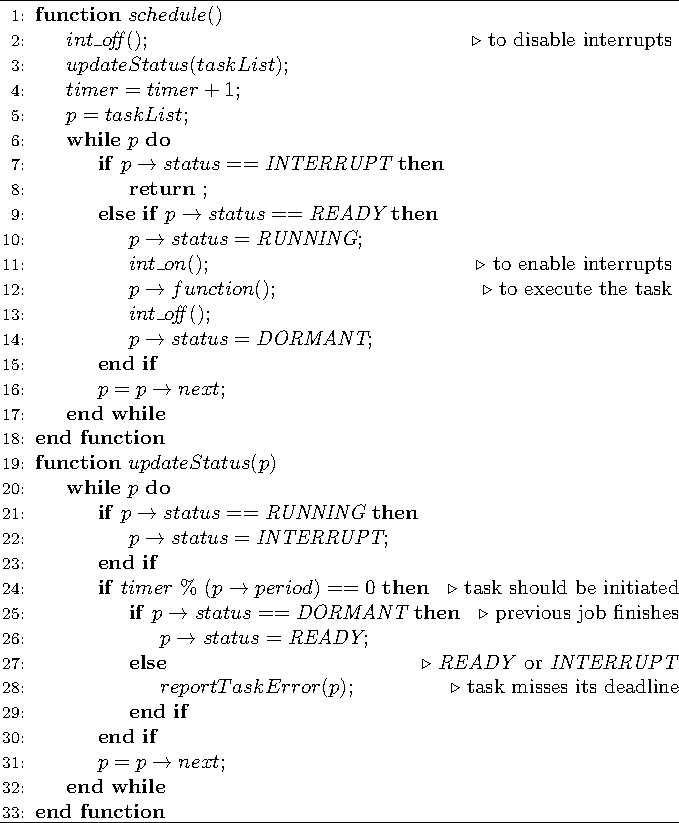
\includegraphics[width=0.9\textwidth]{FIG1_15-TIE-3480.pdf}
\caption{中断处理函数 $\mathit{schedule()}$ 的类 C 伪码}
\label{f:schedule}
\end{figure}

在图~\ref{f:schedule} 展示的伪码中,中断处理函数 $\mathit{schedule()}$ 首先通过调用函数 $\mathit{updateStatus()}$ 更新了 $\mathit{taskList}$ 中所有任务的状态。这个更新的动作,实际上对当前中断周期需要被调度的任务进行了初始化。然后 $\mathit{schedule()}$ 对链表 $\mathit{taskList}$ 进行遍历,对就绪的任务(状态为 \textit{READY})轮流予以执行,或者当遇到一个被中断的任务(状态为 \textit{INTERRUPT}\footnote{需要注意,状态 \textit{INTERRUPT} 表示该任务当前被中断,或者它曾经被中断而它目前仍未运行完毕。})时,进行返回操作(return)。由于 $\mathit{taskList}$ 中的任务是按优先级降序排列的,这样的遍历方式意味着调度从优先级高的任务开始。至于函数 $\mathit{updateStatus()}$,它对每一个任务的更新操作分为两步:首先,如果该任务正在运行(状态为 \textit{RUNNING}),则成为被中断状态;其次,当该任务处于应当进行初始化的时刻,如果该任务的上一个实例已经运行结束(状态为 \textit{DORMANT}),则变成就绪状态,否则意味着它错过了时限,将产生一个错误。需要注意,函数 $\mathit{schedule()}$ 仅仅在中断请求被处理时才会被调用。如果系统处于不可中断状态,即中断屏蔽标志位为 1,该函数则不会被调用。得益于中断屏蔽标志位,当函数 $\mathit{schedule()}$ 正在更新任务状态或寻找下一个该被运行的任务时,它不能被中断。然而,当它正在运行某个周期性任务时(第 12 行),它可以被中断。这就造成了函数 $\mathit{schedule()}$ 可能被嵌套调用。

为简便起见,本文用“调度过程”(scheduling)指代如下阶段:从中断请求被响应的时刻起,到第一个应当被运行的周期性任务开始运行(即图~\ref{f:schedule} 中第 8 行或第 12 行)的时刻止。因此,“调度开销”包括三部分:
\begin{enumerate}
\item 当中断请求被响应时,从正在运行的任务函数切换到 $\mathit{schedule()}$ 函数所耗费的上下文切换时间;
\item $\mathit{schedule()}$ 用于搜索\emph{第一个} 应当被运行的任务,以及准备运行该任务所花费的时间,对应图~\ref{f:schedule} 中第 2--11 行;
\item 从函数 $\mathit{schedule()}$ 切换到应当被运行的任务函数所耗费的上下文切换时间。
\end{enumerate}
“任务切换”(switching)指代以下阶段:从一个周期性任务实例完成其运行的时刻起,到下一个应当被运行的周期性任务开始运行的时刻止。同样,“任务切换开销”也包含三部分:
\begin{enumerate}
\item 当某个周期性任务实例运行完毕时,从该任务函数切换至 $\mathit{schedule()}$ 所耗费的上下文切换时间;
\item $\mathit{schedule()}$ 用于搜索\emph{下一个} 应当被运行的任务,以及准备运行该任务所花费的时间;
\item 从函数 $\mathit{schedule()}$ 切换到应当被运行的任务函数所耗费的上下文切换时间。
\end{enumerate}
 

\subsection{系统建模}
\label{s:formalism}


对硬件平台的部分技术细节(比如中断屏蔽技术)予以考虑,我们假设系统模型满足以下条件:

\begin{enumerate}
\item [(A1')] 任务 $\tau_i$ 的实例初始化时刻,等于在时刻 $kT_i$ 发出的时钟中断请求被响应的时刻,其中整数 $k\ge 0$;
\item [(A2)] 任意任务 $\tau_i$ 的运行时间 $C_i$ 是常数,它不随时间而改变;
\item [(A3)] 所有任务之间互相独立,使得它们在初始化的那一刻就可以被运行,并且随时可被其它任务抢占;
\item [(A4')] 系统的调度开销以及任务切换开销需要在模型中予以考虑,其它系统开销均被忽略。
\end{enumerate}


这些假设条件使我们的模型有别于标准 RMS 模型。比如说,根据假设条件~(A1'),如果中断请求出现在任务切换的过程中,那么它的响应将被推迟,使得 $\tau_i$ 的任务实例不能在时刻 $kT_i$ 进行初始化。它们将被推迟,直到任务切换过程结束时中断屏蔽位被清零。这与假设条件~(A1) 是不一样的。另一方面,条件~(A3) 假定任务实例在初始化时刻就进入就绪状态,随时可以被运行。然而,任何任务实例都不可能在初始化时刻就开始运行,因为调度过程也需要耗时。

\begin{figure}[ht]
\centering
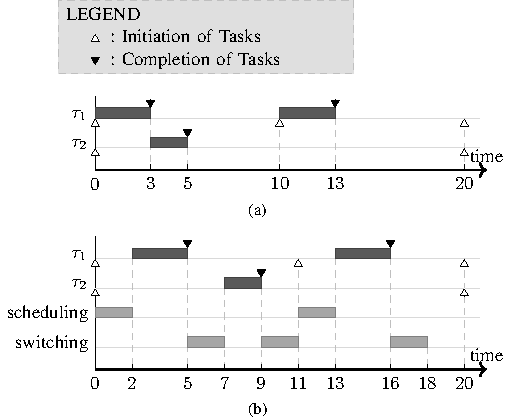
\includegraphics[width=0.7\textwidth]{FIG2_15-TIE-3480.pdf}
\caption{RMS 算法和 RMS 系统实现调度对比}
\label{f:example}
\end{figure}

根据这些假设条件,图~\ref{f:example}(b) 展示了图~\ref{f:example}(a) 的任务集在 RMS 系统实现中被调度的情况,其中假定调度开销和任务切换开销都为 2 个时间单位,时钟中断周期为 10。与图~\ref{f:example}(a) 不同,在图~\ref{f:example}(b) 中,在时刻 0,首先开始被运行的是调度过程。在经过了 2 个时间单位后,调度过程结束,优先级最高的 $\tau_1$ 才开始被运行。在时刻 5,当 $\tau_1$ 运行结束后,系统需要进行长达 2 个时间单位的任务切换,然后在时刻 7,任务 $\tau_2$ 才开始被运行。特别需要注意的是,在时刻 10,虽然有时钟中断请求发生,但因为正处于任务切换过程中,中断请求被屏蔽,中断响应被推迟。直到时刻 11 任务切换结束时,中断请求才被响应。$\tau_1$ 的初始化时刻是 11,而不是 10。这个行为展示了条件~(A1') 与 (A1) 的不同。

在本小节,我们将首先介绍如何利用带类型的项表达式来对系统状态建模,然后展示如何利用重写规则对系统的关键行为进行建模。特别需要指出,系统中的\emph{瞬时行为}(instantaneous  behaviors)将在第~\ref{ss:ir}、\ref{ss:init} 和~\ref{ss:inthandling} 小节进行解释;在第~\ref{ss:timedbehavior} 小节,将对系统的\emph{时间行为}(timed behaviors)进行解释。根据第~\ref{ss:realtime-modeling} 小节所述,系统中涉及时间的行为将利用 $\cR$ 规则进行描述,根据算法~\ref{alg:convert},即利用 Maude 的 $R$ 规则进行建模。

\subsubsection{基本类型}

在建立的系统模型中,任务将由它们在 $\mathit{taskList}$ 中的下标进行标识。所有下标具有自然数类型 \verb|Nat|。我们定义类型 \verb|MaybeNat| 对类型 \verb|Nat| 进行封装,用于指代任务集中的某个周期性任务。类型 \verb|MaybeNat| 具有两个\emph{构造子}(constructor):构造子 \verb|some| 带有类型为 \verb|Nat| 的参数 $n$,表示 $\mathit{taskList}$ 中第 $n$ 个任务;构造子 \verb|none| 指代“没有任务”。
\begin{verbatim}
  op none : -> MaybeNat [ctor] .
  op some_ : Nat -> MaybeNat [ctor] .
\end{verbatim}
其中关键字 \verb|ctor| 表示所对应的函数符号是构造子。

类型 \verb|Stack| 被定义用于对系统的栈结构进行建模。栈中存储的是被中断的任务(编号)。基于类型 \verb|Stack|,我们定义了栈操作 \verb|push|、 \verb|pop| 和 \verb|peek|。

类型 \verb|Counter| 被定义作为计数器,记录某个任务的\emph{已运行时间} 和运行时间。

在实际的代码中,$\mathit{schedule()}$ 函数的全局变量 $\mathit{timer}$ 在达到上界时将会被置 0。这一合理的技术细节没有在图~\ref{f:schedule} 进行展示,但包含在我们的模型中。$\mathit{timer}$ 的上界等于所有任务周期的最小公倍数。类型 \verb|Timer| 被定义用于对 $\mathit{timer}$ 进行建模。

\subsubsection{系统状态的建模}

整个对象系统可看作由以下几部分组成:被调度的任务集;RMS 调度模块;硬件平台,包括寄存器和栈;以及时钟中断源。其中 RMS 调度模块(即函数 $\mathit{schedule()}$)的状态可以只用单一变量 $\mathit{timer}$ 来表示。下面将给出其它部分的状态模型。

\paragraph{任务:} 由于我们的模型只关心调度问题,任务将被抽象成一个类型为 \verb|Counter| 的计数器。因为需要考虑调度过程和任务切换,这两个过程在模型中被当作两个\emph{系统任务}。每一个任务都被建模成基类 \verb|Task| 的某个子类的实例对象:
\begin{verbatim}
  class Task | cnt : Counter .
  op error : -> Object [ctor] .
\end{verbatim}
其中 \verb|error| 是用于表示某任务超时(即错过了时限)的实例对象。

被调度的周期性任务是类 \verb|PTask| 的实例。类 \verb|PTask| 是 \verb|Task| 的子类,具有额外的属性 \verb|priority|(表示任务优先级)、\verb|period|(表示任务周期)和 \verb|status|(表示任务状态):
\begin{verbatim}
  class PTask | priority : Nat, period : Nat, 
                status : Status .
  subclass PTask < Task .
\end{verbatim}
其中类型 \verb|Status| 具有四个常量构造子 \verb|RUNNING|、 \verb|INTERRUPT|、 \verb|READY| 和 \verb|DORMANT|,与图~\ref{f:schedule} 相对应。

周期性任务的链表(即系统实现中的变量 $\mathit{taskList}$)用类型 \verb|TaskList| 进行建模。\verb|TaskList| 是由 \verb|PTask| 的实例对象以及 \verb|error| 对象组成的列表结构。周期性任务由该列表中的元素下标进行标识。

另一方面,系统任务是类 \verb|SysTask| 的实例。类 \verb|SysTask| 也是 \verb|Task| 的子类,但没有额外的属性。与周期性任务不同的是,系统任务的集合具有类型 \verb|SysTasks|,而 \verb|SysTasks| 是多重集而非列表。系统任务由自身的对象标识 \verb|Oid| 进行标识。

\paragraph{硬件:} 我们的系统模型考虑了与中断处理有关的硬件部分——寄存器和栈。

寄存器被建模成类 \verb|Regs| 的实例。该类的属性 \verb|pc| 描述程序计数器 PC(Program Counter),属性 \verb|mask| 表示中断屏蔽标志位,属性 \verb|ir| 表示中断请求标志位: 
\begin{verbatim}
  class Regs | pc : TaskID, 
               mask : Bool, ir : Bool .
\end{verbatim}
其中,类型 \verb|TaskID| 包含子类型 \verb|MaybeNat| 和 \verb|Oid|,用于标识某个任务(包括周期性任务和系统任务)。类 \verb|Regs| 定义了对各属性的操作,如 \verb|getPc| 和 \verb|setMask| 等。 

于是硬件状态被建模成具有类型 \verb|Hardware| 的项表达式。\verb|Hardware| 由两部分构成:类 \verb|Regs| 的一个实例,和类型为 \verb|Stack| 的一个项表达式。

\paragraph{中断源:} 中断源被建模成类 \verb|IntSrc| 的一个实例。类 \verb|IntSrc| 具有两个属性:\verb|cycle| 表示时钟中断周期 $T$;\verb|val| 的数值随着时间推移从 $T$ 递减为 $0$。
\begin{verbatim}
  class IntSrc | val : Time, cycle : Time .
\end{verbatim}

\paragraph{系统状态:} 在我们的模型中,系统状态由以上部分组合构成,具有类型 \verb|System|\footnote{根据 Maude 的使用习惯,变量符号将由大写字母表示。为了易于阅读,变量声明语句在此省略。}:
\begin{verbatim}
  op _____ : TaskList Timer SysTasks 
             Hardware Object ~> System [ctor] .
  mb (L T STS HW < O : IntSrc |>) : System .
\end{verbatim}
其中,“\verb|~>|” 表示该函数符号是个\emph{部分函数}(partial function);关键字 \verb|mb| 声明一种\emph{成员关系}(membership),在这里表示,如果一个项表达式由 \verb|TaskList|(周期任务列表)、\verb|Timer|(变量 $\mathit{timer}$)、\verb|SysTasks|(系统任务集合)、\verb|Hardware|(硬件) 以及类 \verb|IntSrc| (中断源) 的实例构成,那么它具有类型 \verb|System|。

\subsubsection{中断请求}
\label{ss:ir}

当属性 \verb|val| 的值递减为 0 时,中断请求由中断源触发。中断请求每隔周期 $T$ 将会发出一次。请求的动作是瞬间完成的,因此将由以下瞬时条件重写规则进行建模。该规则作用于类型为 \verb|System| 的项表达式:
\begin{verbatim}
  crl [interrupt-request] :
    (L T STS HW ISRC) 
    => (L T STS (HW).intReq reset(ISRC))
    if (ISRC).timeout .
\end{verbatim}
其中,函数 \verb|_.timeout| 检查属性 \verb|val| 的值是否为 0;函数 \verb|_.intReq| 将属性 \verb|ir| 置 1,表示当前存在中断请求需要被响应。

然后该中断请求将等待被响应处理,其过程的建模将在第~\ref{ss:inthandling} 小节进行解释。

\subsubsection{任务初始化}
\label{ss:init}
周期性任务将按顺序被图~\ref{f:schedule} 中的函数 $\mathit{updateStatus()}$ 进行初始化。这一过程在我们的模型中被看作一个瞬时行为。它将由以下函数 \verb|updateStatus_with_| 进行建模:
\begin{verbatim}
  op updateStatus_with_ : TaskList Timer 
                            -> TaskList . 
\end{verbatim}
该函数对 $\mathit{taskList}$ 中的任务逐一应用函数 \verb|update_with_|,使任务状态得到更新(对应图~\ref{f:schedule} 的第 21--30 行):
\begin{verbatim}
  op update_with_ : Object Timer ~> Object .
  ceq update < O : PTask | period : T, 
                           status : ST > 
        with TIMER
      = if ST == DORMANT 
        then < O : PTask | status : READY >
        else error fi
      if TIMER rem T == 0 .
  eq update < O : PTask | status : ST > 
       with TIMER
     = if ST == RUNNING 
       then < O : PTask | status : INTERRUPT >
       else < O : PTask |> fi [otherwise] .
\end{verbatim}
其中变量符号 \verb|TIMER| 表示全局变量 $\mathit{timer}$ 的值。给定一个周期性任务,如果 \verb|TIMER|(即 $\mathit{timer}$)可被任务周期 \verb|T| 整除,那么该任务需要被初始化。在任务需要被初始化的情况下:如果它处于空闲状态(\verb|DORMANT|),则将进入就绪状态(\verb|READY|);否则意味着该任务的上一个任务实例没有运行完毕,因此该任务超时,产生 \verb|error| 对象。在任务不需要被初始化的情况下,只有当其处于运行状态(\verb|RUNNING|)时,任务状态才需要被改变。

通过对比可以看出,模型中的函数 \verb|updateStatus_with_| 具有与图~\ref{f:schedule} 中函数 $\mathit{updateStatus()}$ 相同的行为。

\subsubsection{中断处理与任务调度}
\label{ss:inthandling}

当中断请求发生时,它可能不会马上被系统检测到。中断请求的检测要求中断屏蔽标志位 \verb|mask| 为 0。一旦系统检测到存在中断请求,中断的处理分为两步:首先是硬件对中断信号的处理,比如清空中断请求标志位 \verb|ir|、将当前函数的上下文压栈等;然后是调用中断处理函数 $\mathit{schedule()}$。这个过程用以下瞬时重写规则进行建模:
\begin{verbatim}
  crl [interrupt-handle] :
    SYSTEM 
    => ((SYSTEM).interrupt).startScheduling
    if (SYSTEM).existInt .
\end{verbatim}
其中,函数 \verb|_.existInt| 检查 \verb|mask| 是否为 0 \emph{且} \verb|ir| 为 1。函数 \verb|_.interrupt| 对硬件的中断处理机制进行建模,它进行了四步操作:
\begin{enumerate}[(i)]
\item 清空标志位 \verb|ir|,表示中断请求已被响应;
\item 将当前程序计数器 \verb|pc| 压进栈中,保存被中断的上下文;
\item 将 \verb|pc| 的值设成具有类型 \verb|Oid| 的项表达式 \verb|scheduling|,表示系统正处于调度阶段;
\item 将中断屏蔽标志位 \verb|mask|置 1,屏蔽即将到来的中断请求。
\end{enumerate}

与周期性任务不同,虽然调度过程也作为系统任务被建模成一个计数器 \verb|Counter|,但因其功能过于重要,以至于不能将其功能完全抽象化。我们将调度过程的行为划分为三部分。第一部分包含了调度过程的时间行为。这一部分通过将调度过程看作一个系统任务(类型为 \verb|SysTask|)来描述其时间行为。时间行为的建模将在第~\ref{ss:timedbehavior} 小节中详述。其它两部分共同定义了调度过程的功能。第二部分对应于图~\ref{f:schedule} 的第 3--4 行。它更新了 $\mathit{taskList}$ 的状态并且给 $\mathit{timer}$ 加 1。这一部分行为被建模成函数 \verb|_.startScheduling|。它将在调度过程的开始时刻作为瞬时动作发生,如以下规则 \verb|interrupt-handle| 所示:
\begin{verbatim}
  op _.startScheduling : System -> System .
  eq (L T STS HW ISRC).startScheduling 
     = ((updateStatus L with T) 
        inc(T) STS HW ISRC) .
\end{verbatim}
第三部分对应于图~\ref{f:schedule} 的第 6--11 行,它负责搜索第一个应该被运行的周期性任务,并准备予以执行。这部分行为被建模成函数 \verb|_.finishScheduling|,并在调度过程的结束时刻作为瞬时动作发生:
\begin{verbatim}
  op _.finishScheduling : System -> System .
  eq (L T STS HW ISRC).finishScheduling
     = (L T (finish scheduling in STS) 
        HW ISRC).run1stTask .
\end{verbatim}
其中,函数 \verb|finish_in_| 重置系统任务 \verb|scheduling| 的计数器;函数 \verb|_.run1stTask| 对第 6--11 行建模,从状态为 \verb|INTERRUPT| 或 \verb|READY| 的任务中找到优先级最高的任务,根据其状态分别进行\emph{中断返回}(interrupt return)或执行动作。

当系统任务 \verb|scheduling| 的已运行时间达到它的运行时间时,调度过程结束。我们用以下规则建模这一瞬时行为:
\begin{verbatim}
  crl [scheduling-finish] :
    SYSTEM => (SYSTEM).finishScheduling
    if SYSTEM := (L T STS HW ISRC) 
       /\ (SYSTEM).running == scheduling 
       /\ scheduling isComplete?in STS .
\end{verbatim}
其中,函数 \verb|_.running| 返回当前系统的 \verb|pc| 值,即正在运行的任务标识;而函数 \verb|_isComplete?in_| 检查该任务的已运行时间是否已达到其运行时间。

与调度过程类似,任务切换过程 \verb|switching| 也被划分为时间行为与其功能行为。当正在运行的周期性任务运行结束时,系统任务 \verb|switching| 开始运行,直到自身的已运行时间达到自身的运行时间。两条类似的瞬时规则 \verb|switching-start| 和 \verb|switching-finish| 被用于对任务切换过程的功能行为进行建模。


\subsubsection{系统的时间行为}
\label{ss:timedbehavior}

系统的时间行为由两部分构成:所有任务的运行和时钟中断源的运行。两者可以同时被以下\emph{标准} 的\emph{单元计时规则}~\cite{DBLP:journals/entcs/OlveczkyM07a}(tick rule)所建模\footnote{关键字 \texttt{nonexec} 允许 Real-Time Maude 根据某种策略来应用重写规则。}:
\begin{verbatim}
  crl [tick]:
    {SYSTEM} => {delta(SYSTEM, R)} in time R 
    if R le mte(SYSTEM) [nonexec] .
\end{verbatim}
其中,函数 \verb|delta| 定义了时间推移对系统状态产生的效果;函数 \verb|mte| 表示的是,从当前时刻直至任意瞬时动作\emph{必须} 发生的时刻,系统允许的\emph{最大时间推移量} (Maximum amount of Time allowed to Elapse)。实际上,对系统时间行为建模的关键就在于定义函数 \verb|delta| 和 \verb|mte|。需要注意的是,变量 \verb|R| 相对于我们所指定的时间域\footnote{Real-Time Maude 包含了预定义的模块用于指定时间域是自然数集或是实数集,而这两者分别定义了\emph{离散} 的时间域和\emph{连续} 的时间域。}(time domain)来说是\emph{连续的}(continuous)。

时间推移对我们的目标系统的影响是,它使 \verb|pc| 指定的任务和时钟中断源的状态随着时间推移在向前推进。具体的表现是,当时间向前推移,正在运行的任务的计数器 \verb|cnt| 在递增,而中断源的 \verb|val| 值在递减:
\begin{verbatim}
  ceq delta((L T STS HW ISRC), R)
      = (deltaTask(ID, L, R) 
         T STS HW (deltaIS(ISRC, R)))
      if ID := (HW).getPc /\ ID :: MaybeNat .
\end{verbatim}
其中,规则的最后一个条件表示 \verb|ID| 的类型为 \verb|MaybeNat|,即表示当前正在运行的任务为周期性任务。类似地,如果 \verb|ID| 的类型为 \verb|Oid|,即当前运行的任务为系统任务,那么函数 \verb|deltaTask| 将作用于 \verb|STS| 而非 \verb|L|。

\verb|mte| 取决于下一个强制发生的瞬时动作的时刻。因此,它由三个因素决定:还有多长时间能完成当前正在运行的任务;还有多长时间产生下一个中断请求;当前是否有中断请求被系统检测到。
\begin{verbatim}
  ceq mte(L T STS HW ISRC)
      = minimum(mteTask(ID, L),
                mteIS(ISRC), mteIr(HW))
      if ID := (HW).getPc /\ ID :: MaybeNat .
\end{verbatim}
其中,如果当前存在中断请求被系统检测到,函数 \verb|mteIr| 将返回 0;否则返回 \verb|INF|,表示\emph{无穷}(infinity)。当 \verb|ID| 为类型 \verb|Oid| 时,情况类似。


\subsection{形式化验证}
\label{s:verification}
在本小节,我们针对不同的真实场景,对 RMS 系统的重写模型进行分析。需要注意,得益于 $\mathit{timer}$ 的上界,从任意(合理的)初始状态出发,该模型的可达状态数是有限的。这使得我们可以应用非时控的模型检测器对模型进行形式化验证。

\subsubsection{验证属性}
本案例我们考虑两个验证属性:可调度性和正确性。通过可调度性,我们验证一个给定的周期性任务集合在该 RMS 系统的调度下是否满足可调度性。通过正确性,我们验证该 RMS 系统对周期性任务的调度方式是否按照 RMS 算法的规范进行。

为了验证可调度性,我们定义原子命题 \verb|taskTimeout|。\verb|taskTimeout| 成立的条件是在当前状态中,$\mathit{taskList}$ 包含 \verb|error| 对象,即某个任务发生超时:
\begin{verbatim}
  op taskTimeout : -> Prop [ctor] .
  eq {L T STS HW ISRC} |= taskTimeout 
     = containError(L) .
\end{verbatim}
其中,函数 \verb|containError| 返回 \verb|true| 当且仅当 \verb|L| 中存在 \verb|error|。 可调度性可以被形式化地描述成时序逻辑公式 \verb|[](~taskTimeout)|,它表示命题 \verb|taskTimeout| 总是不成立。由于该性质与时钟无关(clock-unrelated),给定初始状态 \verb|init|,以下非时控模型检测命令可以用于验证可调度性是否在任意时刻总是成立。如果成立,该命令返回 \verb|true|;否则,该命令返回一条反例路径:
\begin{verbatim}
  (mc init |=u [](~taskTimeout) .)
\end{verbatim}

本案例另外一个重要目的是验证该系统实现的正确性。我们定义原子命题 \verb|correct|,它成立的条件是,当前运行的周期性任务是所有请求运行的周期性任务中优先级最高的:
\begin{verbatim}
  op correct : -> Prop [ctor] .
  ceq {L T STS HW ISRC} |= correct
      = if ID :: MaybeNat then shouldRun(ID, L)
        else true fi
      if ID := (HW).getPc .
\end{verbatim}
其中,函数 \verb|shouldRun(ID, L)| 返回 \verb|true| 的条件是,标识为 \verb|ID| 的任务在当前所有非空闲状态的任务中具有最高优先级。需要注意的是,在系统的运行过程中,如果存在任务超时,我们的验证需求不关心任务超时后的行为(比如错误恢复等)。因此,实现正确性可以被以下时序逻辑公式描述:\verb|([]correct)\/(correct U taskTimeout)|,表示 \verb|correct| 总是成立,或者保持成立直到命题 \verb|taskTimeout| 成立。给定初始状态 \verb|init|,正确性能被以下非时控模型检测命令所验证:
\begin{verbatim} 
  (mc init |=u ([]correct) 
               \/ (correct U taskTimeout) .)
\end{verbatim}

\subsubsection{验证场景}
\label{ss:results} 
我们在验证过程中使用以下参数配置,数据来源于我们的工业合作伙伴提供的真实数据:
\begin{itemize}
\item 时钟中断周期 $T$ 为 $5ms$;
\item 调度开销为 $38{\mu}s$,任务切换开销为 $20{\mu}s$;
\item 初始状态的栈为空,程序计数器 \verb|pc| 为空,中断屏蔽标志位 \verb|mask| 为 0,中断请求标志位 \verb|ir| 为 0。
\end{itemize}

我们在 10 种不同的场景下对我们的模型进行了验证。其中既包括我们的合作伙伴提供的真实场景,也包括我们自己设计的实验场景。其中四个场景描述如下:
\begin{itemize}
\item 场景 (i) 包含2个任务 $\tau_1$ 和 $\tau_2$: $T_1=5ms$, $C_1=3ms$, $T_2=25ms$, $C_2=7ms$;
\item 场景 (ii) 包含 2 个任务 $\tau_1$ 和 $\tau_2$: $T_1=5ms$, $C_1=2ms$, $T_2=25ms$, $C_2=2.3ms$;
\item 场景 (iii) 包含 3 个任务 $\tau_1$、$\tau_2$ 和 $\tau_3$:$T_1=5ms$, $C_1=2.7ms$, $T_2=10ms$, $C_2=2ms$, $T_3=25ms$, $C_3=3ms$;
\item 场景 (iv) 包含 3 个任务 $\tau_1$、$\tau_2$ 和 $\tau_3$:$T_1=5ms$, $C_1=2.5ms$, $T_2=10ms$, $C_2=1.5ms$, $T_3=15ms$, $C_3=4.5ms$。
\end{itemize}
值得注意的是,得益于 Real-Time Maude 丰富的表达能力,对不同的任务集合,我们只需要定义不同的初始状态(类型为 \verb|System|)即可,不需要对模型本身进行修改和调整。

在验证的过程中,我们的模型选择了连续的时间域以及\emph{极大时间采样策略}(maximal time sampling strategy)。模型检测的结果显示,正确性在所有场景中成立。而对于可调度性,它在场景 (i--iii) 成立,但在场景 (iv) 中不成立。我们将模型检测命令返回的反例路径绘成图~\ref{f:counterexample}。从图中可以看到,在第 $15ms$ 时,任务 $\tau_3$ 的第一个实例还没有完成运行,而此时它的第二个任务实例进行初始化,于是发生了超时,可调度性不成立。

\hide{
以上结果展示了我们的方法在真实工业系统中的可用性。然而,为了检验此方法的效率,我们进一步尝试将我们的方法应用于规模更大的实验场景中。
实验场景完全随机产生。我们在上述参数配置下验证随机实验场景的可调度性。进行验证的机器配置为:英特尔酷睿 2 Quad Q9550,2.83GHz,4 核,8GB 内存,64 位 Ubuntu
15.04 操作系统。 在50个随机生成的包含5个周期性任务的实验场景中,我们发现各场景的验证时间差别极大,从 $300ms$ 到超时(超时时间设为90分钟)不等。
这是由于模型检测的效率取决于状态空间的规模。而在我们的模型中,状态空间的规模与
 $mn$ 正相关,其中 $m$ 是变量 $\mathit{timer}$ 的上界,$n$ 是周期任务的数量。
对这些随机实验场景的验证结果表明,我们的方法在90分钟内能处理的场景规模大约为 $mn$ 等于  $10^6$。
}

\subsubsection{结果评估}
本小节将说明我们的验证结果是可靠且完备的。

给定一个验证方法,如果这个方法产生的任何反例都是原问题的真正反例,则称这个验证方法是\emph{可靠的};如果应用该方法没有找到反例,能说明原问题也不存在反例,则称这个验证方法是\emph{完备的}。要判断我们的方法是否可靠很简单,只需要检查产生的反例是否真反例。比如,图~\ref{f:counterexample} 的反例是真反例,这表明关于场景~(iv) 可调度性的验证结果是可靠的。然而需要证明完备性,却不太简单。我们的模型选择了连续时间域,使其行为更加贴近真实系统。然而这一选择也导致了系统的状态空间成为无穷大,不可能穷尽所有状态。

一般来说,我们没有办法证明非时控的模型检测方法对任意系统、任意时间采样策略以及任意验证属性都具有完备性。然而, \"Olveczky 和 Meseguer 证明了非时控的时序逻辑模型检测方法,在应用极大时间采样策略对“某类”实时系统进行“某类”LTL 公式的验证时,是完备的~\cite{DBLP:journals/entcs/OlveczkyM07a}。“这类”实时系统称作\emph{时间鲁棒的}(time-robust),而“这类”LTL 公式由\emph{单元计时不变的}(tick-invariant)命题构成\footnote{在此我们避免引入时间鲁棒性和单元计时不变性的准确定义,因为这需要更深入的重写逻辑背景知识。}。

\begin{landscape}
\begin{figure}[t]
\centering 
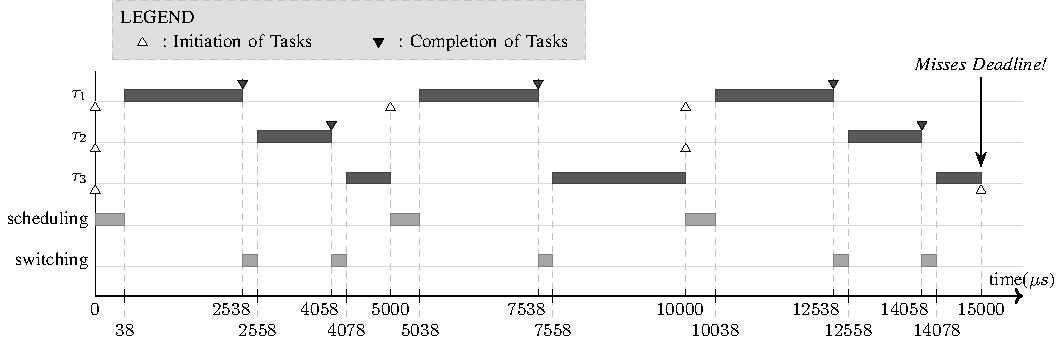
\includegraphics[width=1.5\textwidth]{FIG3_15-TIE-3480.pdf}
\caption{场景 (iv) 可调度性的反例}
\label{f:counterexample}
\end{figure}
\end{landscape}

\begin{theorem}[\inlinecite{DBLP:journals/entcs/OlveczkyM07a}]
\label{t:completeness}
给定一个时间鲁棒的实时重写逻辑模型 $\mathcal{R}^{\cL}$,一个单元计时不变的原子命题集合 $AP$,一个由 $AP$ 中命题构成的 LTL 公式 $\Phi$ (不包含 $\bigcirc$ 操作符)。那么非时控的时序逻辑模型检测方法在应用极大时间采样策略对 $\Phi$ 进行验证时,它是\emph{完备的}。
\end{theorem}

因此,我们可以证明以下定理,表明第~\ref{ss:results} 小节的验证结果是完备的。
\begin{theorem}
\label{t:main}
采用非时控模型检测方法去验证本案例的系统模型的可调度性和正确性,所得结果是完备的。
\end{theorem}
\begin{proof}
首先证明我们的模型是时间鲁棒的;其次证明我们定义的原子命题 \verb|taskTimeout| 和 \verb|correct| 是单元计时不变的;最后应用定理~\ref{t:completeness} 得到结论。更详细的证明,请参见附录~\ref{app:proof}。
\end{proof}


\subsection{相关工作}
\label{s:relate}
在本小节,我们从三个方面来对本案例应用及其相关工作进行对比。

先从可调度性判定的角度来说,Liu 和 Layland 给出了一个最常用的充分条件:一个周期性任务集合如果满足 $\Sigma^n_{i=1} C_i/T_i \le n(2^{1/n}-1)$,那么它根据 RMS 算法是可调度的~\cite{DBLP:journals/jacm/LiuL73}。然后,Bini 等人提出了一个更有效的充分条件~\cite{DBLP:journals/tc/BiniBB03},它具有跟前者同样的算法复杂度。在另一方面,判定可调度性的充分必要条件由 Sprunt 等人~\cite{DBLP:journals/rts/SpruntSL89} 及 Audsley 等人~\cite{audsley1993deadline} 分别提出,要求对任务集合进行更复杂的分析。然而,所有这些分析都建立在理想的模型上,并不考虑系统开销,真实性不如本文建立的模型。Katcher 等人基于几种主流的 RMS 实现方法,在可调度性分析中考虑了系统开销~\cite{DBLP:journals/tse/KatcherAS93}。然而,本案例的目标系统不在他们的考虑范围之内。此外,相比于那些理论的分析,本文采用的基于形式化建模与验证的分析方法主要有三个优点。一是如果我们的可调度性检查给出系统“不可调度”的结果,它同时能够返回一条反例路径。这条反例路径可以指导开发人员调整系统设计,比如调整任务优先级、甚至改变调度算法。第二个优点是,如果想要在系统中应用一个全新的调度策略,本小节的分析方法只需要对模型进行修改就能对新策略进行分析,而理论分析方法则需要重新进行分析和推理。最后一个优点是,在分析中考虑系统开销和硬件细节会给模型引入不确定性。比如在我们的模型中,如果正在运行的任务\emph{恰好} 在中断请求发生时完成运行,则将可能发生两种不同的行为:(i)~系统进行任务切换,在任务切换过程中中断请求被屏蔽,因此调度过程和任务的初始化将被推迟;(ii)~系统立即响应该中断请求,则任务切换将被推迟。相比于本案例的自动验证方法,对这些不确定行为进行理论分析要复杂得多。

Tian 和 Duan~\cite{TianD2011} 以及 Cui 等人~\cite{DBLP:conf/iceccs/CuiDT14} 以类似的方法,利用模型检测技术对 RMS 算法进行了分析。与本案例不同的是,这两项工作使用了不同的建模语言和工具。Tian 和 Duan 使用 SPIN~\cite{DBLP:journals/tse/Holzmann97} 的一类扩展对 RMS 算法进行建模和验证~\cite{TianD2011};而 Cui 等人则使用了逻辑编程语言 TMSVL~\cite{DBLP:conf/icfem/HanDW12} 及其模型检测工具~\cite{DBLP:conf/iceccs/CuiDT14}。这两项工作与本工作存在两个主要区别。首先,最重要的区别在于,这两项工作的分析对象都是 RMS 算法的标准理想模型~\cite{DBLP:journals/jacm/LiuL73},而不是包含了更多复杂细节的系统实现,这也是本案例应用的主要出发点。实际上,如果我们假设调度过程和任务切换的时间等于 0,那么标准的 RMS 模型将成为我们的 RMS 系统模型的特例。因此,本案例建立的模型更具一般性。另外一个区别在于,如果需要在周期任务集合中添加一个新任务,Tian 和 Duan 的模型~\cite{TianD2011} 以及 Cui 等人的模型~\cite{DBLP:conf/iceccs/CuiDT14} 都需要进行修改,为新任务及其行为增加一个子模块。特别需要指出的是,Tian 和 Duan 模型中的调度部分同样需要调整以增加新任务~\cite{TianD2011}。然而,在我们的模型中,增加新任务只需要修改初始状态即可,模型不需作任何修改。这一点已经在第~\ref{ss:results} 小节中指出。另一方面,Tian 和 Duan 在模型中使用离散时间域~\cite{TianD2011},而我们的模型则使用了参数化的时间域,允许实例化成离散时间域或连续时间域,非常灵活。Cui 等人也使用了连续的时间域,同时采用建模策略以减少状态空间规模~\cite{DBLP:conf/iceccs/CuiDT14},与本工作的极大时间采样策略类似。但我们证明了此方法的完备性(定理~\ref{t:main}),而 Cui 等人没有给出类似结论。

最后, Maude 和 Real-Time Maude 目前已成功地被应用到诸多领域~\cite{DBLP:journals/jlp/Meseguer12},特别是通信协议、安全协议。但还没有被应用于分析调度问题。据我们所知,这是首次利用 Real-Time Maude 分析 RMS 算法及其实现。


\subsection{案例小结}
\label{s:conclusion}
在本案例应用中,我们利用 Real-Time Maude 对一个真实的 RMS 系统进行了建模。在建立的系统模型中,我们考虑了调度及任务切换所产生的系统开销,也考虑了硬件平台的部分细节。我们的模型包含了足够多的细节对真实的目标系统行为进行描述。通过对建立的模型应用模型检测技术,我们在不同的关键场景下验证了系统的可调度性和正确性。最后我们证明了验证结果是可靠且完备的。该系统目前在某工业级航天控制器中在线运行。


\section{本章小结}

本章基于已有的重写逻辑建模验证工作,针对嵌入式系统的特性,如结构层次化、高度并发、并发行为与顺序行为并存、系统结构动态变化、实时性等,提出了基于规范化条件重写模型的建模方法。通过模型层面的语义映射,我们将该建模方法在工具集 Maude 中予以实现。利用该方法,我们对两个真实的嵌入式系统——机车优化控制系统和速率单调调度系统进行了建模分析。对于前者,我们应用了测试与验证结合的方法,成功发现系统中的潜在缺陷;该系统目前运行稳定,并在
沈阳铁路局通过了实车运用考核。而对于后者,我们应用模型检测技术对系统的可调度性和正确性进行了形式化验证,并证明了其结果具有可靠性和完备性;经验证的系统目前在某工业级航天控制器中在线运行。这两个应用案例表明了本章提出的建模方法在实际应用中具有可行性。
